\documentclass[11pt,a4paper]{article}

\usepackage[utf8]{inputenc}
\usepackage[T1]{fontenc}
\usepackage{lmodern}
\usepackage{geometry}
\usepackage{graphicx}
\usepackage{booktabs}
\usepackage{array}
\usepackage{longtable}
\usepackage{tabularx}
\usepackage{xcolor}
\usepackage{hyperref}
\usepackage{listings}
\usepackage{fancyhdr}
\usepackage{titlesec}
\usepackage{enumitem}
\usepackage{tikz}
\usepackage{float}
\usepackage{caption}
\usepackage{subcaption}
\usepackage{amsmath}
\usepackage{multirow}
\usepackage{tcolorbox}
\usepackage{pifont}
\usepackage{xltabular}
\usetikzlibrary{positioning, shapes, arrows.meta, fit, backgrounds, calc}

\geometry{margin=1in, top=1.2in, bottom=1.2in}

\definecolor{UNBBlue}{RGB}{0,40,85}
\definecolor{UNBLightBlue}{RGB}{100,150,200}
\definecolor{UNBGray}{RGB}{128,128,128}
\definecolor{UNBLightGray}{RGB}{245,245,245}
\definecolor{UNBGreen}{RGB}{39,174,96}
\definecolor{UNBRed}{RGB}{231,76,60}
\definecolor{UNBOrange}{RGB}{243,156,18}
\definecolor{CodeBg}{RGB}{248,248,248}

\hypersetup{
    colorlinks=true,
    linkcolor=UNBBlue,
    urlcolor=UNBBlue,
    citecolor=UNBBlue,
}

\pagestyle{fancy}
\fancyhf{}
\fancyhead[L]{\small\textcolor{UNBGray}{CloudWatch AI -- Implementation Report}}
\fancyhead[R]{\small\textcolor{UNBGray}{CS6905 -- Winter 2026}}
\fancyfoot[C]{\thepage}
\renewcommand{\headrulewidth}{0.4pt}
\renewcommand{\footrulewidth}{0pt}

\titleformat{\section}
  {\Large\bfseries\color{UNBBlue}}{\thesection}{1em}{}[\vspace{-0.3em}\textcolor{UNBBlue}{\rule{\textwidth}{0.5pt}}]
\titleformat{\subsection}
  {\large\bfseries\color{UNBBlue}}{\thesubsection}{1em}{}
\titleformat{\subsubsection}
  {\normalsize\bfseries\color{UNBBlue}}{\thesubsubsection}{1em}{}

\lstdefinestyle{codestyle}{
    backgroundcolor=\color{CodeBg},
    basicstyle=\ttfamily\footnotesize,
    breaklines=true,
    frame=single,
    rulecolor=\color{UNBLightBlue},
    framesep=6pt,
    xleftmargin=8pt,
    xrightmargin=8pt,
    showstringspaces=false,
    keywordstyle=\color{UNBBlue}\bfseries,
    commentstyle=\color{UNBGray}\itshape,
    stringstyle=\color{UNBGreen},
    numbers=none,
    captionpos=b,
}
\lstset{style=codestyle}

\tcbuselibrary{skins, breakable}

\newtcolorbox{infobox}[1][]{
  colback=blue!5,
  colframe=UNBBlue,
  fonttitle=\bfseries,
  title=#1,
  boxrule=0.5pt,
  arc=2pt,
  left=6pt,
  right=6pt,
  top=4pt,
  bottom=4pt,
}

\newtcolorbox{successbox}[1][]{
  colback=green!5,
  colframe=UNBGreen,
  fonttitle=\bfseries,
  title=#1,
  boxrule=0.5pt,
  arc=2pt,
  left=6pt,
  right=6pt,
  top=4pt,
  bottom=4pt,
}

\newtcolorbox{warnbox}[1][]{
  colback=orange!5,
  colframe=UNBOrange,
  fonttitle=\bfseries,
  title=#1,
  boxrule=0.5pt,
  arc=2pt,
  left=6pt,
  right=6pt,
  top=4pt,
  bottom=4pt,
}

% Checkmark and crossmark
\newcommand{\cmark}{\textcolor{UNBGreen}{\ding{51}}}
\newcommand{\xmark}{\textcolor{UNBRed}{\ding{55}}}

\begin{document}

% ========================
% TITLE PAGE
% ========================
\begin{titlepage}
\begin{center}

\vspace*{1.5cm}

{\Huge\bfseries\textcolor{UNBBlue}{CloudWatch AI}}\\[0.5cm]
{\LARGE\textcolor{UNBBlue}{Implementation Report}}\\[0.3cm]
{\large Real-Time AIOps Platform for Predictive Incident Detection}

\vspace{1.5cm}

\textcolor{UNBBlue}{\rule{0.8\textwidth}{0.5pt}}

\vspace{1.5cm}

{\large
\textbf{Course:} CS6905 -- Cloud Information Management Systems\\[0.3cm]
\textbf{Instructor:} Dr.\ Shadi Aljendi\\[0.3cm]
\textbf{University of New Brunswick}
}

\vspace{1.5cm}

{\large
\begin{tabular}{ll}
\textbf{Team Members:} & Alfarizy Alfarizy (3810253) \\
                        & Akinbobola Akin (3784664) \\
                        & Ishimwe Pacis Hanyurwimfura (3787234)
\end{tabular}
}

\vspace{1.5cm}

{\large\textbf{Date:} March 30, 2026}

\vspace{1cm}

\textcolor{UNBBlue}{\rule{0.8\textwidth}{0.5pt}}

\vfill

{\small
\textbf{Repository:} \url{https://github.com/helloimrizy-pages/cloud-project}\\[0.2cm]
\textbf{Live Dashboard:} \url{http://cloud-project-dashboard1.s3-website-us-east-1.amazonaws.com}\\[0.2cm]
\textbf{API Endpoint:} \texttt{https://p9fpx4nhh6.execute-api.ca-central-1.amazonaws.com}
}

\end{center}
\end{titlepage}

% ========================
% TABLE OF CONTENTS
% ========================
\tableofcontents
\newpage

% ========================
% SECTION 1: EXECUTIVE SUMMARY
% ========================
\section{Executive Summary}

CloudWatch AI is a serverless AIOps platform we built to predict cloud service incidents before they actually occur. We designed and deployed the entire solution on AWS, training Gradient Boosting machine learning models on 2.4 million timesteps of cloud service KPI data. In practice, the system delivers early warnings at \textbf{0.91 precision} with a \textbf{$\sim$36-minute average lead time}, and it produces fewer than one false alarm per service per day.

\begin{infobox}[Key Achievements]
\begin{itemize}[leftmargin=1em, itemsep=2pt]
    \item \textbf{13 Lambda functions} that handle everything from data ingestion to the REST API
    \item \textbf{6 DynamoDB tables} with Streams configured for event-driven processing
    \item \textbf{19 JWT-protected API routes} served through API Gateway
    \item \textbf{5 monitored cloud services} that are running real-time simulations across \textbf{6 scenarios}
    \item \textbf{3 ML models}, one for each prediction horizon (5, 10, and 15 minutes)
    \item \textbf{Per-user data isolation} through Cognito-based \texttt{owner\_id} partitioning on every table
    \item \textbf{Email alert notifications} via Amazon SNS that is filtered on a per-user basis
    \item \textbf{React 19 dashboard} with 4 interactive pages, auto-polling, and a dark/light theme toggle
    \item \textbf{AWS Cognito authentication} using the SRP protocol with email verification
    \item \textbf{OWASP Top 10 audit}: 9 out of 10 passed, 1 not applicable (overall risk: Low)
    \item \textbf{50+ integration test cases} for all system layers
\end{itemize}
\end{infobox}

Taken together, the platform shows what a complete, production-grade cloud database application looks like end to end, from data generation and ML inference all the way through to real-time visualization and security hardening. Every component runs serverlessly within the AWS Free Tier in the \texttt{ca-central-1} region.

% ========================
% SECTION 2: ARCHITECTURE IMPLEMENTATION
% ========================
\section{Architecture Implementation}

\subsection{Architecture Overview}

We structured CloudWatch AI around a \textbf{serverless, event-driven architecture} on AWS. By relying entirely on managed services at every layer, we avoided server provisioning altogether. The system scales on its own and keeps costs low since we only pay for what we actually use.

\begin{figure}[H]
\centering
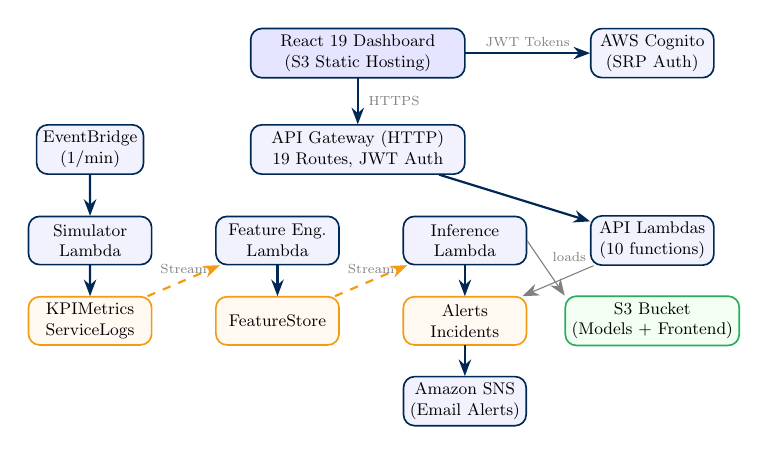
\begin{tikzpicture}[
  scale=0.68, transform shape,
  box/.style={rectangle, rounded corners=4pt, draw=UNBBlue, fill=blue!5, minimum width=2.3cm, minimum height=0.9cm, font=\small, align=center, line width=0.6pt},
  dbbox/.style={rectangle, rounded corners=4pt, draw=UNBOrange, fill=orange!5, minimum width=2.3cm, minimum height=0.9cm, font=\small, align=center, line width=0.6pt},
  s3box/.style={rectangle, rounded corners=4pt, draw=UNBGreen, fill=green!5, minimum width=2.3cm, minimum height=0.9cm, font=\small, align=center, line width=0.6pt},
  arrow/.style={-{Stealth[length=6pt]}, thick, UNBBlue},
  stream/.style={-{Stealth[length=6pt]}, thick, UNBOrange, dashed},
  label/.style={font=\scriptsize, UNBGray}
]

% Row 1: User + Frontend
\node[box, minimum width=4cm, fill=blue!10] (browser) at (0,5) {React 19 Dashboard\\(S3 Static Hosting)};
\node[box] (cognito) at (5.5,5) {AWS Cognito\\(SRP Auth)};

% Row 2: API Gateway
\node[box, minimum width=4cm] (apigw) at (0,3.2) {API Gateway (HTTP)\\19 Routes, JWT Auth};

% Row 3: Lambda functions
\node[box] (simulator) at (-5,1.5) {Simulator\\Lambda};
\node[box] (feateng) at (-1.5,1.5) {Feature Eng.\\Lambda};
\node[box] (inference) at (2,1.5) {Inference\\Lambda};
\node[box] (apilambda) at (5.5,1.5) {API Lambdas\\(10 functions)};

% Row 4: Data stores
\node[dbbox] (kpi) at (-5,0) {KPIMetrics\\ServiceLogs};
\node[dbbox] (features) at (-1.5,0) {FeatureStore};
\node[dbbox] (alerts) at (2,0) {Alerts\\Incidents};
\node[s3box] (s3) at (5.5,0) {S3 Bucket\\(Models + Frontend)};

% EventBridge
\node[box, minimum width=1.8cm] (eventbridge) at (-5,3.2) {EventBridge\\(1/min)};

% Arrows
\draw[arrow] (browser) -- node[label, right, xshift=2pt] {HTTPS} (apigw);
\draw[arrow] (browser) -- node[label, above] {JWT Tokens} (cognito);
\draw[arrow] (apigw) -- (apilambda);
\draw[arrow] (eventbridge) -- (simulator);

% Data flow
\draw[arrow] (simulator) -- (kpi);
\draw[stream] (kpi) -- node[label, above] {Stream} (feateng);
\draw[arrow] (feateng) -- (features);
\draw[stream] (features) -- node[label, above] {Stream} (inference);
\draw[arrow] (inference) -- (alerts);
\draw[arrow, thin, gray] (inference.east) -- node[label, above right] {\scriptsize loads} (s3.north west);

% SNS
\node[box, minimum width=1.8cm] (sns) at (2,-1.5) {Amazon SNS\\(Email Alerts)};
\draw[arrow] (alerts) -- (sns);

% API reads
\draw[arrow, gray, thin] (apilambda) -- (alerts);

\end{tikzpicture}
\captionsetup{justification=centering}
\caption{System Architecture. Solid arrows indicate direct calls; dashed orange arrows indicate DynamoDB Stream triggers.}
\label{fig:architecture}
\end{figure}

\subsection{Cloud Infrastructure Components}

Everything is deployed in the \texttt{ca-central-1} (Canada -- Central) AWS region. Table~\ref{tab:aws-services} gives a full inventory of every AWS service we used along with its configuration.

\begin{table}[H]
\centering
\begin{tabular}{lll}
\toprule
\textbf{Service} & \textbf{Configuration} & \textbf{Purpose} \\
\midrule
AWS Lambda & 13 functions (Python 3.11/3.12) & Compute \\
Amazon DynamoDB & 6 tables, on-demand capacity & Database \\
Amazon API Gateway & HTTP API, 19 routes & REST API \\
Amazon SNS & 1 topic (CloudWatchAI-Alerts) & Email notifications \\
Amazon S3 & 1 bucket & Static hosting + model storage \\
Amazon EventBridge & 1 rule (rate: 1 minute) & Simulation scheduler \\
Amazon Cognito & 1 User Pool (``CloudWatchAI'') & Authentication \\
Amazon ECR & 1 container image & Inference Lambda image \\
Amazon CloudWatch & Logs for all Lambda functions & Monitoring \\
\bottomrule
\end{tabular}
\caption{AWS Service Inventory}
\label{tab:aws-services}
\end{table}

\subsection{Lambda Functions}

We deployed 13 Lambda functions in total, which we confirmed by running \texttt{aws lambda list-functions}. Table~\ref{tab:lambda-functions} lists each one.

\begin{table}[H]
\centering
\begin{tabular}{llll}
\toprule
\textbf{Function Name} & \textbf{Runtime} & \textbf{Trigger} & \textbf{Memory} \\
\midrule
\texttt{simulator\_lambda} & Python 3.12 & EventBridge (1/min) & 128 MB \\
\texttt{feature\_engineering\_lambda} & Python 3.11 & DynamoDB Stream & 128 MB \\
\texttt{inference\_lambda} & Docker (Python 3.11) & DynamoDB Stream & 512 MB \\
\texttt{services\_lambda} & Python 3.12 & API Gateway & 128 MB \\
\texttt{kpi\_lambda} & Python 3.12 & API Gateway & 128 MB \\
\texttt{alerts\_lambda} & Python 3.12 & API Gateway & 128 MB \\
\texttt{incidents\_lambda} & Python 3.12 & API Gateway & 128 MB \\
\texttt{analytics\_lambda} & Python 3.12 & API Gateway & 128 MB \\
\texttt{threshold\_lambda} & Python 3.12 & API Gateway & 128 MB \\
\texttt{control\_simulation\_lambda} & Python 3.12 & API Gateway & 128 MB \\
\texttt{get\_metrics\_lambda} & Python 3.12 & API Gateway & 128 MB \\
\texttt{get\_logs\_lambda} & Python 3.12 & API Gateway & 128 MB \\
\texttt{notifications\_lambda} & Python 3.12 & API Gateway & 128 MB \\
\bottomrule
\end{tabular}
\caption{Lambda Functions (verified from AWS)}
\label{tab:lambda-functions}
\end{table}

We had to package the \texttt{inference\_lambda} as a Docker container image (pushed to ECR) because its dependencies, scikit-learn, numpy, scipy, and pandas, exceed Lambda's standard 250 MB deployment package size limit.

\subsection{S3 Bucket Configuration}

We use a single S3 bucket for the whole project:

\begin{enumerate}[leftmargin=2em]
    \item \textbf{\texttt{cloud-project-dashboard1}} -- This bucket hosts the compiled React frontend (with static website hosting turned on) and also stores our trained ML models:
    \begin{itemize}
        \item \texttt{index.html}, \texttt{assets/} -- the frontend build output
        \item \texttt{models/model\_h5.pkl} (139.9 KB), \texttt{model\_h10.pkl} (139.6 KB), \texttt{model\_h15.pkl} (139.9 KB)
        \item \texttt{models/thresholds.json} (2.6 KB), \texttt{models/feature\_importances.json} (662 B)
    \end{itemize}
\end{enumerate}

We turned on S3 encryption (AES-256, SSE-S3) with BucketKey optimization. For SPA routing, the static website hosting configuration sets \texttt{ErrorDocument = index.html} so that React Router can handle all client-side paths.

\begin{figure}[H]
\centering
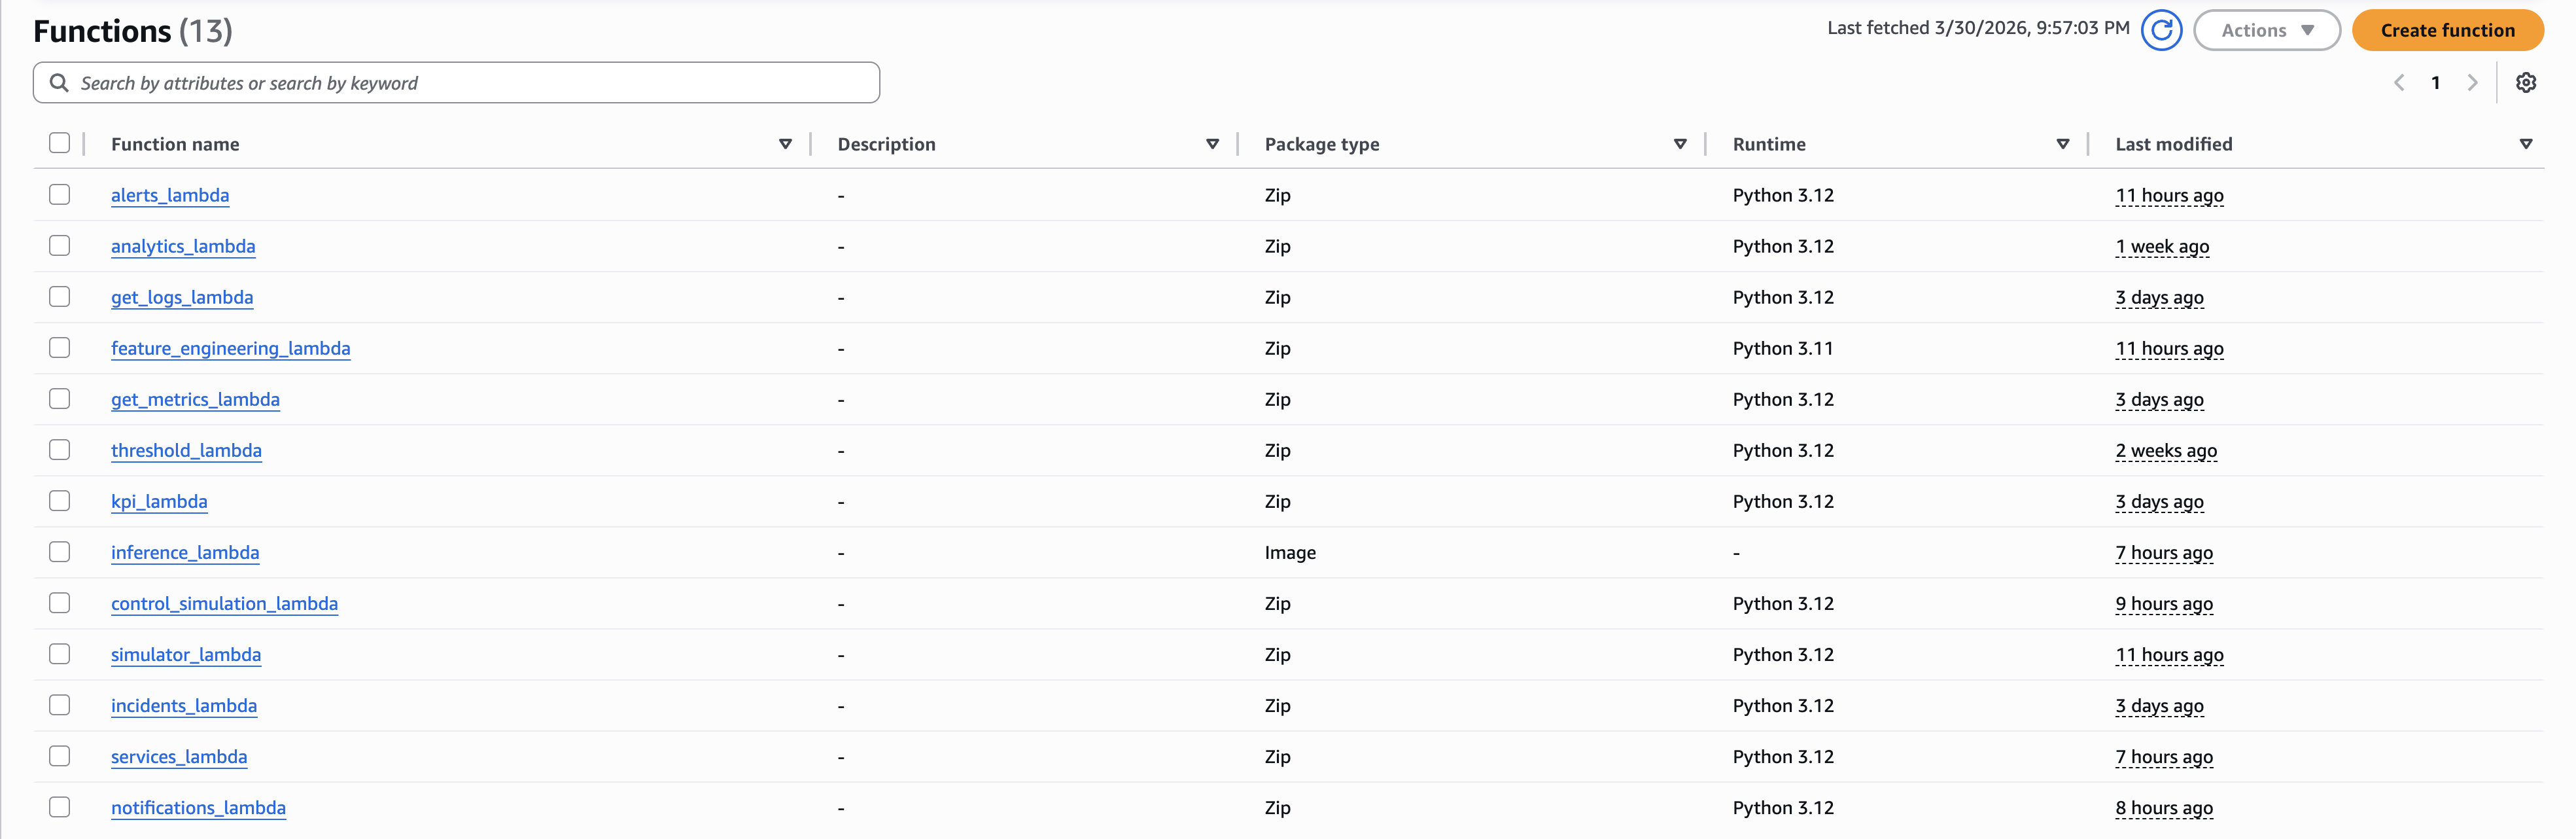
\includegraphics[width=0.9\linewidth]{images/lambda_console.png}
\caption{AWS Lambda Console -- 13 deployed functions}
\label{fig:lambda-console}
\end{figure}

\begin{figure}[H]
\centering
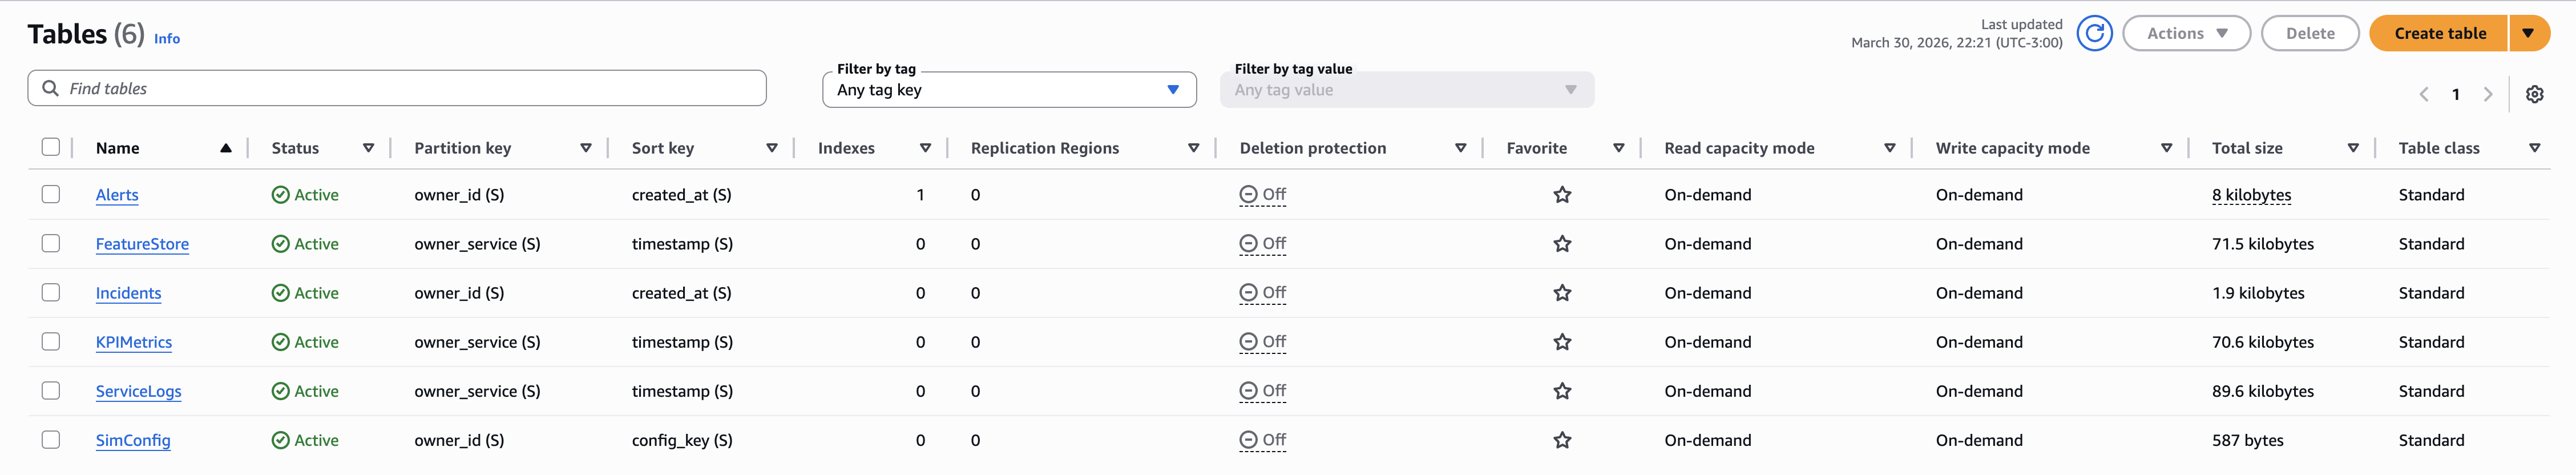
\includegraphics[width=1.0\linewidth]{images/dynamodb_tables.png}
\caption{AWS DynamoDB Console -- 6 tables}
\label{fig:dynamo-console}
\end{figure}

% ========================
% SECTION 3: DATABASE SETUP
% ========================
\section{Database Setup}

\subsection{DynamoDB Table Design}

We went with Amazon DynamoDB as our NoSQL database for a pretty practical reason: each of our 5 monitored cloud services produces \textbf{a completely different JSON structure}. Had we gone with a relational database, we would have needed lots of nullable columns or entirely separate tables for every service type. DynamoDB's flexible document schema lets us store records with different shapes in the same table, and we never have to worry about schema migrations.

Table~\ref{tab:dynamo-tables} shows all 6 DynamoDB tables along with their key schemas and what each one does. We verified these on March 30, 2026 using \texttt{aws dynamodb describe-table}.

\begin{table}[H]
\centering
\begin{tabular}{lllp{4.2cm}}
\toprule
\textbf{Table} & \textbf{Partition Key} & \textbf{Sort Key} & \textbf{Purpose} \\
\midrule
KPIMetrics & \texttt{owner\_service} (S) & \texttt{timestamp} (S) & Raw service metrics, isolated per user \\
ServiceLogs & \texttt{owner\_service} (S) & \texttt{timestamp} (S) & Event logs, isolated per user \\
FeatureStore & \texttt{owner\_service} (S) & \texttt{timestamp} (S) & 8 computed features \\
Alerts & \texttt{owner\_id} (S) & \texttt{created\_at} (S) & Prediction alerts (GSI on \texttt{owner\_status}) \\
Incidents & \texttt{owner\_id} (S) & \texttt{created\_at} (S) & Grouped incidents \\
SimConfig & \texttt{owner\_id} (S) & \texttt{config\_key} (S) & Per-user simulation state \\
\bottomrule
\end{tabular}
\caption{DynamoDB Tables (verified from AWS)}
\label{tab:dynamo-tables}
\end{table}

\subsection{Per-User Data Isolation}

One of our core requirements was making sure that each authenticated user can only see their own simulation data, alerts, and incidents, nobody else's. To accomplish this, we embedded the Cognito \texttt{sub} (the user ID) directly into every table's partition key:

\begin{itemize}[leftmargin=2em]
    \item For the \textbf{data tables} (KPIMetrics, ServiceLogs, FeatureStore), we created a composite partition key: \texttt{owner\_service = \{owner\_id\}\#\{service\_id\}}. That way, each user's service data lives in its own physical partition, and there is no risk of cross-user leakage.
    \item \textbf{Alerts and Incidents} use \texttt{owner\_id} directly as the partition key. We also added a GSI (\texttt{GSI\_AlertsByOwnerStatus}) on the Alerts table, keyed by \texttt{owner\_status} (which concatenates \texttt{\{owner\_id\}\#\{severity\}}), so we can run filtered queries efficiently.
    \item \textbf{SimConfig} also uses \texttt{owner\_id} as its partition key, which means different users can run their simulations concurrently without interfering with each other.
    \item On the API side, every Lambda function pulls \texttt{owner\_id} out of the JWT claims (specifically \texttt{requestContext.authorizer.jwt.claims.sub}) and scopes all database queries to that user.
\end{itemize}

\subsection{Key Design Choices}

\begin{enumerate}[leftmargin=2em]
    \item \textbf{Partition Key = \texttt{owner\_service}}: We chose the composite key \texttt{\{owner\_id\}\#\{service\_id\}} as the partition key for our data tables. It bundles per-user isolation and per-service querying into a single key, which matches the most frequent access pattern we have: ``give me all the data for one specific service belonging to one specific user.''
    \item \textbf{Sort Key = \texttt{timestamp}}: With timestamp as the sort key, we can efficiently run time-range queries within a single partition, for instance, pulling the last 30 minutes of KPI data for \texttt{web-api-001}.
    \item \textbf{TTL (Time To Live)}: Every data table has a \texttt{ttl} attribute that we set to 24 hours. DynamoDB takes care of deleting expired records on its own, so storage costs stay low and we do not need any cleanup scripts.
    \item \textbf{DynamoDB Streams}: We turned on Streams for both the \texttt{KPIMetrics} and \texttt{FeatureStore} tables, using the \texttt{NEW\_IMAGE} view type. Whenever a new record lands in one of these tables, the stream event fires off the next Lambda in the pipeline, Feature Engineering or Inference, respectively. This gives us a fully event-driven pipeline without writing any orchestration logic.
    \item \textbf{On-demand capacity}: All of our tables run in on-demand billing mode. They scale up and down automatically with the workload, which suits us well because the simulation load varies quite a bit.
\end{enumerate}

\subsection{Variable Schema per Service}

The real payoff of DynamoDB is that it can store documents with different structures side by side in the same table. Table~\ref{tab:service-fields} illustrates the distinct fields that each of our five service types generates.

\begin{table}[H]
\centering
\begin{tabular}{ll}
\toprule
\textbf{Service} & \textbf{Unique JSON Fields} \\
\midrule
Web API & \texttt{response\_time\_ms}, \texttt{requests\_per\_second}, \texttt{error\_rate}, \texttt{http\_5xx\_count} \\
DB Pool & \texttt{active\_connections}, \texttt{query\_duration\_avg\_ms}, \texttt{deadlock\_count} \\
Message Queue & \texttt{queue\_depth}, \texttt{consumer\_lag}, \texttt{dead\_letter\_queue\_size} \\
Auth Service & \texttt{login\_success\_rate}, \texttt{auth\_latency\_ms}, \texttt{mfa\_challenge\_rate} \\
ML Pipeline & \texttt{inference\_latency\_ms}, \texttt{model\_accuracy}, \texttt{data\_drift\_score} \\
\bottomrule
\end{tabular}
\caption{Service-Specific KPI Fields in KPIMetrics Table}
\label{tab:service-fields}
\end{table}

\subsection{Sample Data}

During each simulation run, the simulator Lambda fills all tables with realistic data. Every record carries the user's \texttt{owner\_id} and the composite \texttt{owner\_service} key to maintain isolation. Here is what a typical \texttt{KPIMetrics} record looks like for the Web API service:

\begin{lstlisting}[language=bash, caption={Sample KPIMetrics item for Web API (from DynamoDB)}]
{
  "owner_service": "ec1d85f8-...-30647aad6e2b#web-api-001",
  "owner_id": "ec1d85f8-...-30647aad6e2b",
  "service_id": "web-api-001",
  "timestamp": "2026-03-30T14:04:46+00:00",
  "service_type": "web_api",
  "scenario_phase": "Normal",
  "simulator_tick": 0,
  "metrics": {
    "response_time_ms": 95,
    "requests_per_second": 450,
    "error_rate": 0.01,
    "http_5xx_count": 1
  },
  "ttl": 1774965886
}
\end{lstlisting}

\begin{figure}[H]
\centering
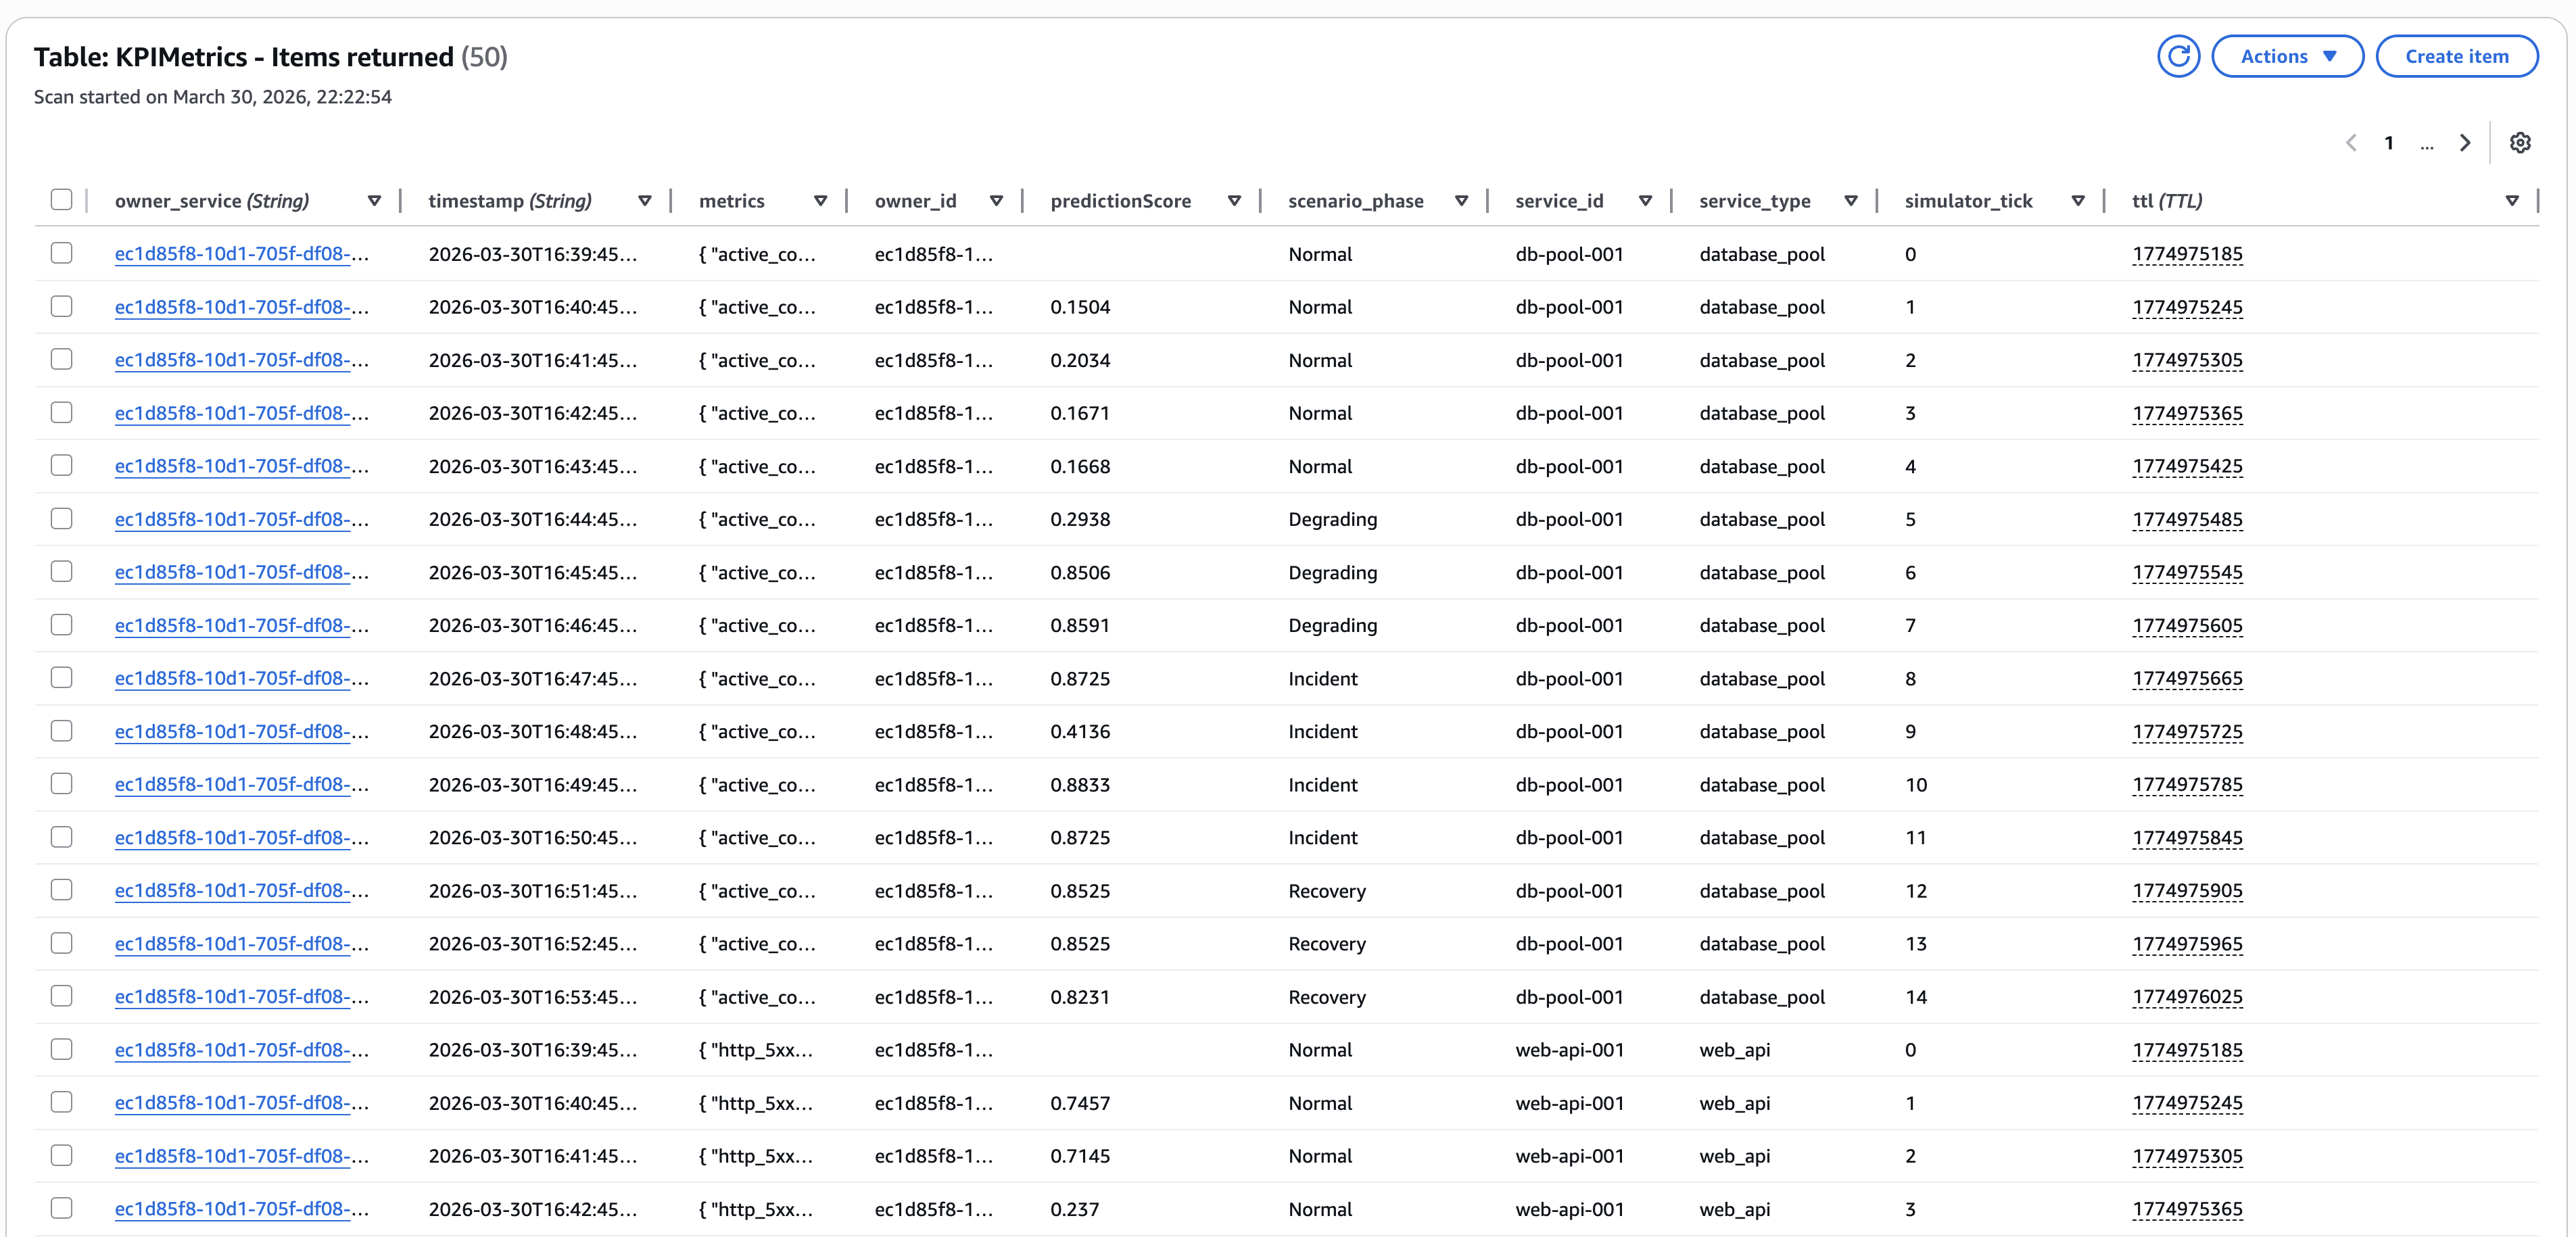
\includegraphics[width=1.0\linewidth]{images/kpi_metrics_table.png}
\caption{DynamoDB KPIMetrics Table -- sample items showing variable schema per service}
\label{fig:dynamo-items}
\end{figure}

% ========================
% SECTION 4: API AND BACKEND DEVELOPMENT
% ========================
\section{API and Backend Development}

\subsection{API Gateway Configuration}

We expose our API through an \textbf{AWS API Gateway HTTP API}, available at:

\begin{center}
\texttt{https://p9fpx4nhh6.execute-api.ca-central-1.amazonaws.com}
\end{center}

Every single one of the 19 routes sits behind a \textbf{JWT Authorizer} that is linked to our Cognito User Pool. We also configured CORS to allow \texttt{GET}, \texttt{POST}, and \texttt{OPTIONS} methods, along with the \texttt{content-type} and \texttt{authorization} headers.

\begin{table}[H]
\centering
\begin{tabular}{lll}
\toprule
\textbf{Method} & \textbf{Route} & \textbf{Description} \\
\midrule
GET & \texttt{/services} & List 5 monitored services with current status \\
GET & \texttt{/kpi/\{serviceId\}} & KPI time-series data for a specific service \\
GET & \texttt{/thresholds} & Alert thresholds per prediction horizon \\
GET & \texttt{/alerts/active} & Active (unresolved) alerts \\
GET & \texttt{/alerts/history} & Historical alerts \\
POST & \texttt{/alerts/\{id\}/acknowledge} & Acknowledge an alert \\
GET & \texttt{/incidents} & Grouped incident objects \\
GET & \texttt{/simulation/state} & Current simulation status \\
POST & \texttt{/simulation/start} & Start simulation with scenario \\
POST & \texttt{/simulation/stop} & Stop running simulation \\
GET & \texttt{/analytics/summary} & Model performance summary \\
GET & \texttt{/analytics/methods} & Model comparison data \\
GET & \texttt{/analytics/features} & Feature importance rankings \\
GET & \texttt{/analytics/lead-times} & Lead time distribution per horizon \\
GET & \texttt{/metrics} & Raw metric records \\
GET & \texttt{/logs} & Service log records \\
GET & \texttt{/notifications/status} & Email subscription status \\
POST & \texttt{/notifications/subscribe} & Subscribe to email alerts \\
POST & \texttt{/notifications/unsubscribe} & Unsubscribe from email alerts \\
\bottomrule
\end{tabular}
\caption{API Routes (all JWT-protected, verified from AWS)}
\label{tab:api-routes}
\end{table}

\subsection{Authorization Verification}

If you try to hit any endpoint without a valid token, you get an HTTP 401 right away:

\begin{lstlisting}[language=bash, caption={JWT Authorization verification}]
$ curl -s https://p9fpx4nhh6.execute-api.ca-central-1.amazonaws.com/services
{"message":"Unauthorized"}
# HTTP 401 -- JWT token required
\end{lstlisting}

\subsection{Simulation Scenarios}

Our simulator supports \textbf{6 configurable scenarios}, and each one exercises a different failure mode across the 5 monitored services. With the exception of the baseline (which stays Normal throughout), all scenarios follow a 15-tick timeline broken into 4 phases: Normal (ticks 0--4), Degrading (5--7), Incident (8--11), and Recovery (12--14).

\begin{table}[H]
\centering
\begin{tabular}{lll}
\toprule
\textbf{Scenario} & \textbf{Primary Service} & \textbf{Also Affected} \\
\midrule
Web API Degradation & web-api-001 & db-pool-001 \\
DB Cascade Failure & db-pool-001 & web-api-001, mq-001 \\
Message Queue Backlog & mq-001 & web-api-001 \\
Auth Service Failure & auth-001 & web-api-001 \\
ML Pipeline Drift & ml-pipeline-001 & -- \\
Normal Operations & -- (all healthy) & -- \\
\bottomrule
\end{tabular}
\caption{Simulation Scenarios}
\label{tab:scenarios}
\end{table}

During the Degrading and Incident phases, each scenario injects realistic metric degradation into the affected services. To give a concrete example: the \textit{Auth Service Failure} scenario gradually pushes the login success rate down from 0.97 to 0.88 while tripling auth latency. Meanwhile, the \textit{ML Pipeline Drift} scenario ramps the data drift score up from 0.05 to 0.20 and simultaneously decreases model accuracy. Services that are not involved in a particular scenario keep emitting normal-range metrics with some jitter, which gives the ML model a realistic mixture of healthy and degraded signals to work with.

\subsection{Data Pipeline (Event-Driven)}

The part of our backend that we are most proud of is the \textbf{fully automatic, event-driven data pipeline} built on top of DynamoDB Streams. There is no polling anywhere, and we did not have to write any orchestration code. Every Lambda in the pipeline also carries the \texttt{owner\_id} forward to keep per-user data isolation intact:

\begin{enumerate}[leftmargin=2em]
    \item \textbf{EventBridge} fires the \texttt{simulator\_lambda} once every 60 seconds. The simulator checks the \texttt{SimConfig} table for all currently active simulations (each keyed by \texttt{owner\_id}) and generates data independently for each user.
    \item The simulator writes KPI metrics and logs for all 5 services into the \texttt{KPIMetrics} and \texttt{ServiceLogs} tables. It uses the composite key \texttt{owner\_service = \{owner\_id\}\#\{service\_id\}} for every record.
    \item As soon as new records land in \texttt{KPIMetrics}, a \textbf{DynamoDB Stream} kicks off the \newline \texttt{feature\_engineering\_lambda}. This function reads the \texttt{owner\_service} and \texttt{owner\_id} from the stream record, computes 8 rolling features, and writes the result to \texttt{FeatureStore} under the same composite key.
    \item The same pattern repeats one level deeper: a \textbf{DynamoDB Stream} on \texttt{FeatureStore} triggers the \texttt{inference\_lambda}. It loads 3 Gradient Boosting models from S3, runs predictions, and, if the score exceeds the calibrated threshold, creates an alert in the \texttt{Alerts} table (keyed by \texttt{owner\_id} + \texttt{created\_at}).
    \item Whenever 2 or more related alerts show up for the same \texttt{owner\_id}, they get grouped into an \texttt{Incident} record.
\end{enumerate}

\subsection{Inference Lambda Implementation}

The inference function ended up being the most complex Lambda in the entire system. Here are the implementation details worth highlighting:

\begin{itemize}[leftmargin=2em]
    \item We had to use \textbf{Docker deployment} because scikit-learn, numpy, and scipy together blow past Lambda's 250 MB deployment limit. The Dockerfile is straightforward:
\end{itemize}

\begin{lstlisting}[language=bash, caption={Inference Lambda Dockerfile}]
FROM --platform=linux/amd64 public.ecr.aws/lambda/python:3.11
RUN pip install "scikit-learn==1.7.2" "numpy<2.3" "scipy<1.15" \
    "joblib" "pandas" boto3 --no-cache-dir
COPY lambda_function.py ${LAMBDA_TASK_ROOT}/
CMD ["lambda_function.handler"]
\end{lstlisting}

\begin{itemize}[leftmargin=2em]
    \item \textbf{Model caching}: During the first (cold) invocation, the Lambda downloads the three models from S3 and saves them in a global \texttt{\_models} dictionary. On subsequent warm invocations, it just reuses what is already in memory, which eliminates the need for repeated downloads.
    \item \textbf{Feature extraction}: The function reads the 8-feature vector from the DynamoDB Stream event that is always in the same fixed order: \texttt{roll\_mean}, \texttt{roll\_max}, \texttt{roll\_std}, \texttt{roll\_slope}, \texttt{first\_diff}, \texttt{error\_rate}, \texttt{warn\_rate}, \texttt{severity\_change\_flag}.
    \item \textbf{Prediction}: For each feature vector that comes in, the Lambda calls \texttt{model.predict\_proba(X)[0, 1]} on all 3 models (one per horizon: 5, 10, 15 minutes).
    \item \textbf{Alert creation}: When the predicted \texttt{score > threshold}, the Lambda creates an alert with a unique ID (\texttt{ALT-XXXXXX}). It classifies severity as CRITICAL when the score is at or above 0.92, and WARNING when it is at or above the threshold but below 0.92. Each alert gets a 24-hour TTL.
    \item \textbf{Email notifications}: Whenever a new alert is created, the Lambda publishes a message to our SNS topic. The \texttt{owner\_id} goes in as a message attribute, so only users who have opted in receive the notification with SNS filter policies handle the routing.
    \item \textbf{Incident grouping}: If there are 2 or more active alerts within a 5-minute window for the same user, they are bundled into an incident (\texttt{INC-XXXXXX}).
\end{itemize}

\subsection{Sample API Responses}

Below are real API responses we captured during a testing session on March 22, 2026:

\begin{lstlisting}[language=bash, caption={GET /services -- returns 5 monitored services}]
[
  {"id":"web-api-001","name":"Web API","type":"API Gateway",
   "status":"healthy","metricName":"Response Time","metricUnit":"ms",
   "currentValue":85},
  {"id":"db-pool-001","name":"DB Pool","type":"Database Pool",
   "status":"warning","metricName":"Query Duration","metricUnit":"ms",
   "currentValue":76},
  {"id":"mq-001","name":"Message Queue","type":"Message Queue",
   "status":"healthy","metricName":"Queue Depth","metricUnit":"messages",
   "currentValue":69},
  {"id":"auth-001","name":"Auth Service","type":"Authentication",
   "status":"healthy","metricName":"Auth Latency","metricUnit":"ms",
   "currentValue":50},
  {"id":"ml-pipeline-001","name":"ML Pipeline","type":"ML Service",
   "status":"healthy","metricName":"Inference Latency","metricUnit":"ms",
   "currentValue":114}
]
\end{lstlisting}

\begin{lstlisting}[language=bash, caption={GET /thresholds -- calibrated per-horizon alert thresholds}]
{"5": 0.912, "10": 0.867, "15": 0.847}
\end{lstlisting}

\begin{lstlisting}[language=bash, caption={GET /analytics/summary -- model performance metrics}]
{"bestPrecision":0.91,"meanLeadTime":36,"falseAlarmRate":"<=1/day",
 "detectionRate":8.7}
\end{lstlisting}

% ========================
% SECTION 5: FRONTEND INTEGRATION
% ========================
\section{Frontend Integration}

\subsection{Technology Stack}

Our dashboard is a \textbf{React 19 single-page application} that we built with TypeScript, Vite 7, Tailwind CSS 4, and Recharts 3.8. The compiled output is hosted as a static website on S3.

\begin{table}[H]
\centering
\begin{tabular}{lll}
\toprule
\textbf{Package} & \textbf{Version} & \textbf{Purpose} \\
\midrule
\texttt{react} & 19.2.0 & UI framework \\
\texttt{react-dom} & 19.2.0 & DOM rendering \\
\texttt{react-router-dom} & 7.13.1 & Client-side routing \\
\texttt{recharts} & 3.8.0 & Interactive charts \\
\texttt{tailwindcss} & 4.2.1 & Utility-first CSS \\
\texttt{amazon-cognito-identity-js} & 6.3.16 & Cognito authentication \\
\texttt{typescript} & $\sim$5.9.3 & Type safety \\
\texttt{vite} & 7.3.1 & Build tool + dev server \\
\bottomrule
\end{tabular}
\caption{Frontend Dependencies (from \texttt{package.json})}
\label{tab:frontend-deps}
\end{table}

\subsection{Application Pages}

The dashboard has 4 main pages plus a login page. Everything is routed client-side:

\subsubsection{Page 1: Live Controls (\texttt{/})}

This is the main dashboard page, and it is where users control simulations in real time:
\begin{itemize}[leftmargin=2em]
    \item A \textbf{scenario selector} dropdown lets users pick from 6 scenarios: \textit{Web API Degradation}, \textit{DB Cascade Failure}, \textit{Message Queue Backlog}, \textit{Auth Service Failure}, \textit{ML Pipeline Drift}, and \textit{Normal Operations}
    \item \textbf{Start/Stop buttons} send \texttt{POST /simulation/start} and \texttt{POST /simulation/stop} requests, showing loading feedback (``Starting...''/``Stopping...'') while the request is in flight
    \item \textbf{4 summary cards} at the top show the current scenario, phase, tick progress, and prediction count
    \item A grid of \textbf{5 Service Health Cards} displays each service's name, type, a color-coded status badge (healthy/warning/critical), current metric value, and unit
\end{itemize}

\subsubsection{Page 2: KPI Timeline (\texttt{/timeline})}

This page is where we show real-time metric visualization such as the following:
\begin{itemize}[leftmargin=2em]
    \item \textbf{Service tabs} let the user switch between viewing an individual service or an ``All Services'' overlay
    \item The \textbf{KPI Value chart} is a Recharts \texttt{LineChart} with shaded reference areas, which indicates warning and danger zones
    \item A separate \textbf{Prediction Score chart} overlays prediction scores alongside a threshold reference line
    \item A \textbf{horizon toggle} switches between the 5m, 10m, and 15m thresholds (0.912, 0.867, 0.847)
    \item In \textbf{All Services mode}, the dashboard fetches data for all 5 services in parallel using \texttt{Promise.all} and overlays lines with distinct colors and a shared legend
\end{itemize}

\subsubsection{Page 3: Alerts \& Incidents (\texttt{/alerts})}

Here users manage alerts and track incidents:
\begin{itemize}[leftmargin=2em]
    \item Each \textbf{active alert card} shows the severity badge (CRITICAL/WARNING/INFO, color-coded), prediction score, threshold, horizon, lead time, and a description
    \item Clicking \textbf{Acknowledge} fires a \texttt{POST /alerts/\{id\}/acknowledge} request, and the card updates to reflect ``Acknowledged'' status
    \item A \textbf{Dismiss button} removes the alert from the visible list (this is purely client-side)
    \item The \textbf{incident timeline} is rendered as a colored horizontal bar showing the scenario phases, with a legend underneath
    \item An \textbf{alert history} section (collapsible) shows previously resolved alerts
    \item An \textbf{email notification toggle} lets users subscribe or unsubscribe to alert emails via SNS. It shows the user's email, subscription status, and whether a confirmation is still pending
    \item Alert timestamps are \textbf{converted to the user's local timezone} using \texttt{toLocaleString()}
\end{itemize}

\subsubsection{Page 4: Analytics (\texttt{/analytics})}

This page focuses on visualizing our model's performance:
\begin{itemize}[leftmargin=2em]
    \item \textbf{4 stat cards} across the top: Best Precision (0.91), Mean Lead Time (36m), False Alarm Rate ($\leq$1/day), Detection Rate (8.7\%)
    \item A \textbf{Precision vs Detection Rate} scatter chart (Recharts \texttt{ScatterChart}) compares our four methods, GBC+Logs, GBC Only, Static Threshold, and Moving Average, across all horizons
    \item The \textbf{Lead Time Distribution} bar chart breaks down min/Q1/median/Q3/max for each horizon
    \item A \textbf{Feature Importance} horizontal bar chart ranks the 8 features, colored by type (KPI features in blue, Log-proxy features in red)
\end{itemize}

\subsection{Authentication Flow}

For authentication, the frontend talks to AWS Cognito through the \texttt{amazon-cognito-identity-js} SDK. The flow works like this:

\begin{enumerate}[leftmargin=2em]
    \item The user types in their email and password on the \texttt{/login} page
    \item Under the hood, the SDK performs an \textbf{SRP (Secure Remote Password)} handshake with Cognito, importantly, the password is never sent over the wire in plaintext
    \item Cognito sends back JWT tokens (ID Token valid for 1 hour, Refresh Token valid for 30 days)
    \item A \texttt{useAuth} context hook makes the user state available throughout the app
    \item Our API client (\texttt{lib/api.ts}) automatically attaches the ID token as an \texttt{Authorization} header on every outgoing request
    \item A \texttt{ProtectedRoute} component wraps all authenticated pages, if there is no valid session, it redirects to \texttt{/login}
    \item If any API call comes back with a 401, the app automatically kicks the user back to the login page
\end{enumerate}

\subsection{Theme System}

We built in support for \textbf{dark and light themes}, and the user's choice persists across sessions:

\begin{itemize}[leftmargin=2em]
    \item A \texttt{useTheme} context hook manages the theme state
    \item Switching themes sets a \texttt{data-theme} attribute on the document root, which toggles a set of CSS variables (\texttt{-{}-color-bg-primary}, \texttt{-{}-color-text-primary}, etc.)
    \item Charts also respect the active theme, we wrote a \texttt{chartColors()} utility that reads CSS custom properties at render time, so Recharts picks up the correct colors automatically
    \item The selected theme is saved to \texttt{localStorage} and restored on page load
    \item To avoid a flash of the wrong color scheme, an inline script in \texttt{index.html} applies the stored theme before React even mounts
\end{itemize}

\subsection{API Integration}

All API calls flow through a single centralized client (\texttt{lib/api.ts}). Here is what it does:

\begin{itemize}[leftmargin=2em]
    \item It reads the API base URL from \texttt{VITE\_API\_BASE\_URL} in production. During development, it falls back to \texttt{/api} (which Vite proxies for us)
    \item Every request gets the Cognito ID token injected as an \texttt{Authorization} header, no manual intervention needed
    \item A 401 response from the API triggers an automatic redirect to the login page
    \item Our custom \texttt{useApi} hook provides \texttt{data}, \texttt{loading}, \texttt{error}, and \texttt{refetch} states. When a component unmounts, in-flight requests are cancelled to prevent memory leaks
    \item \textbf{Auto-polling}: The \texttt{useApi} hook takes an optional \texttt{pollInterval} parameter (we set it to 5 seconds for the live pages). Polling pauses when the browser tab is hidden (\texttt{document.hidden} check), and it skips a tick if the previous request has not finished yet, so requests never pile up
\end{itemize}

\begin{figure}[H]
\centering
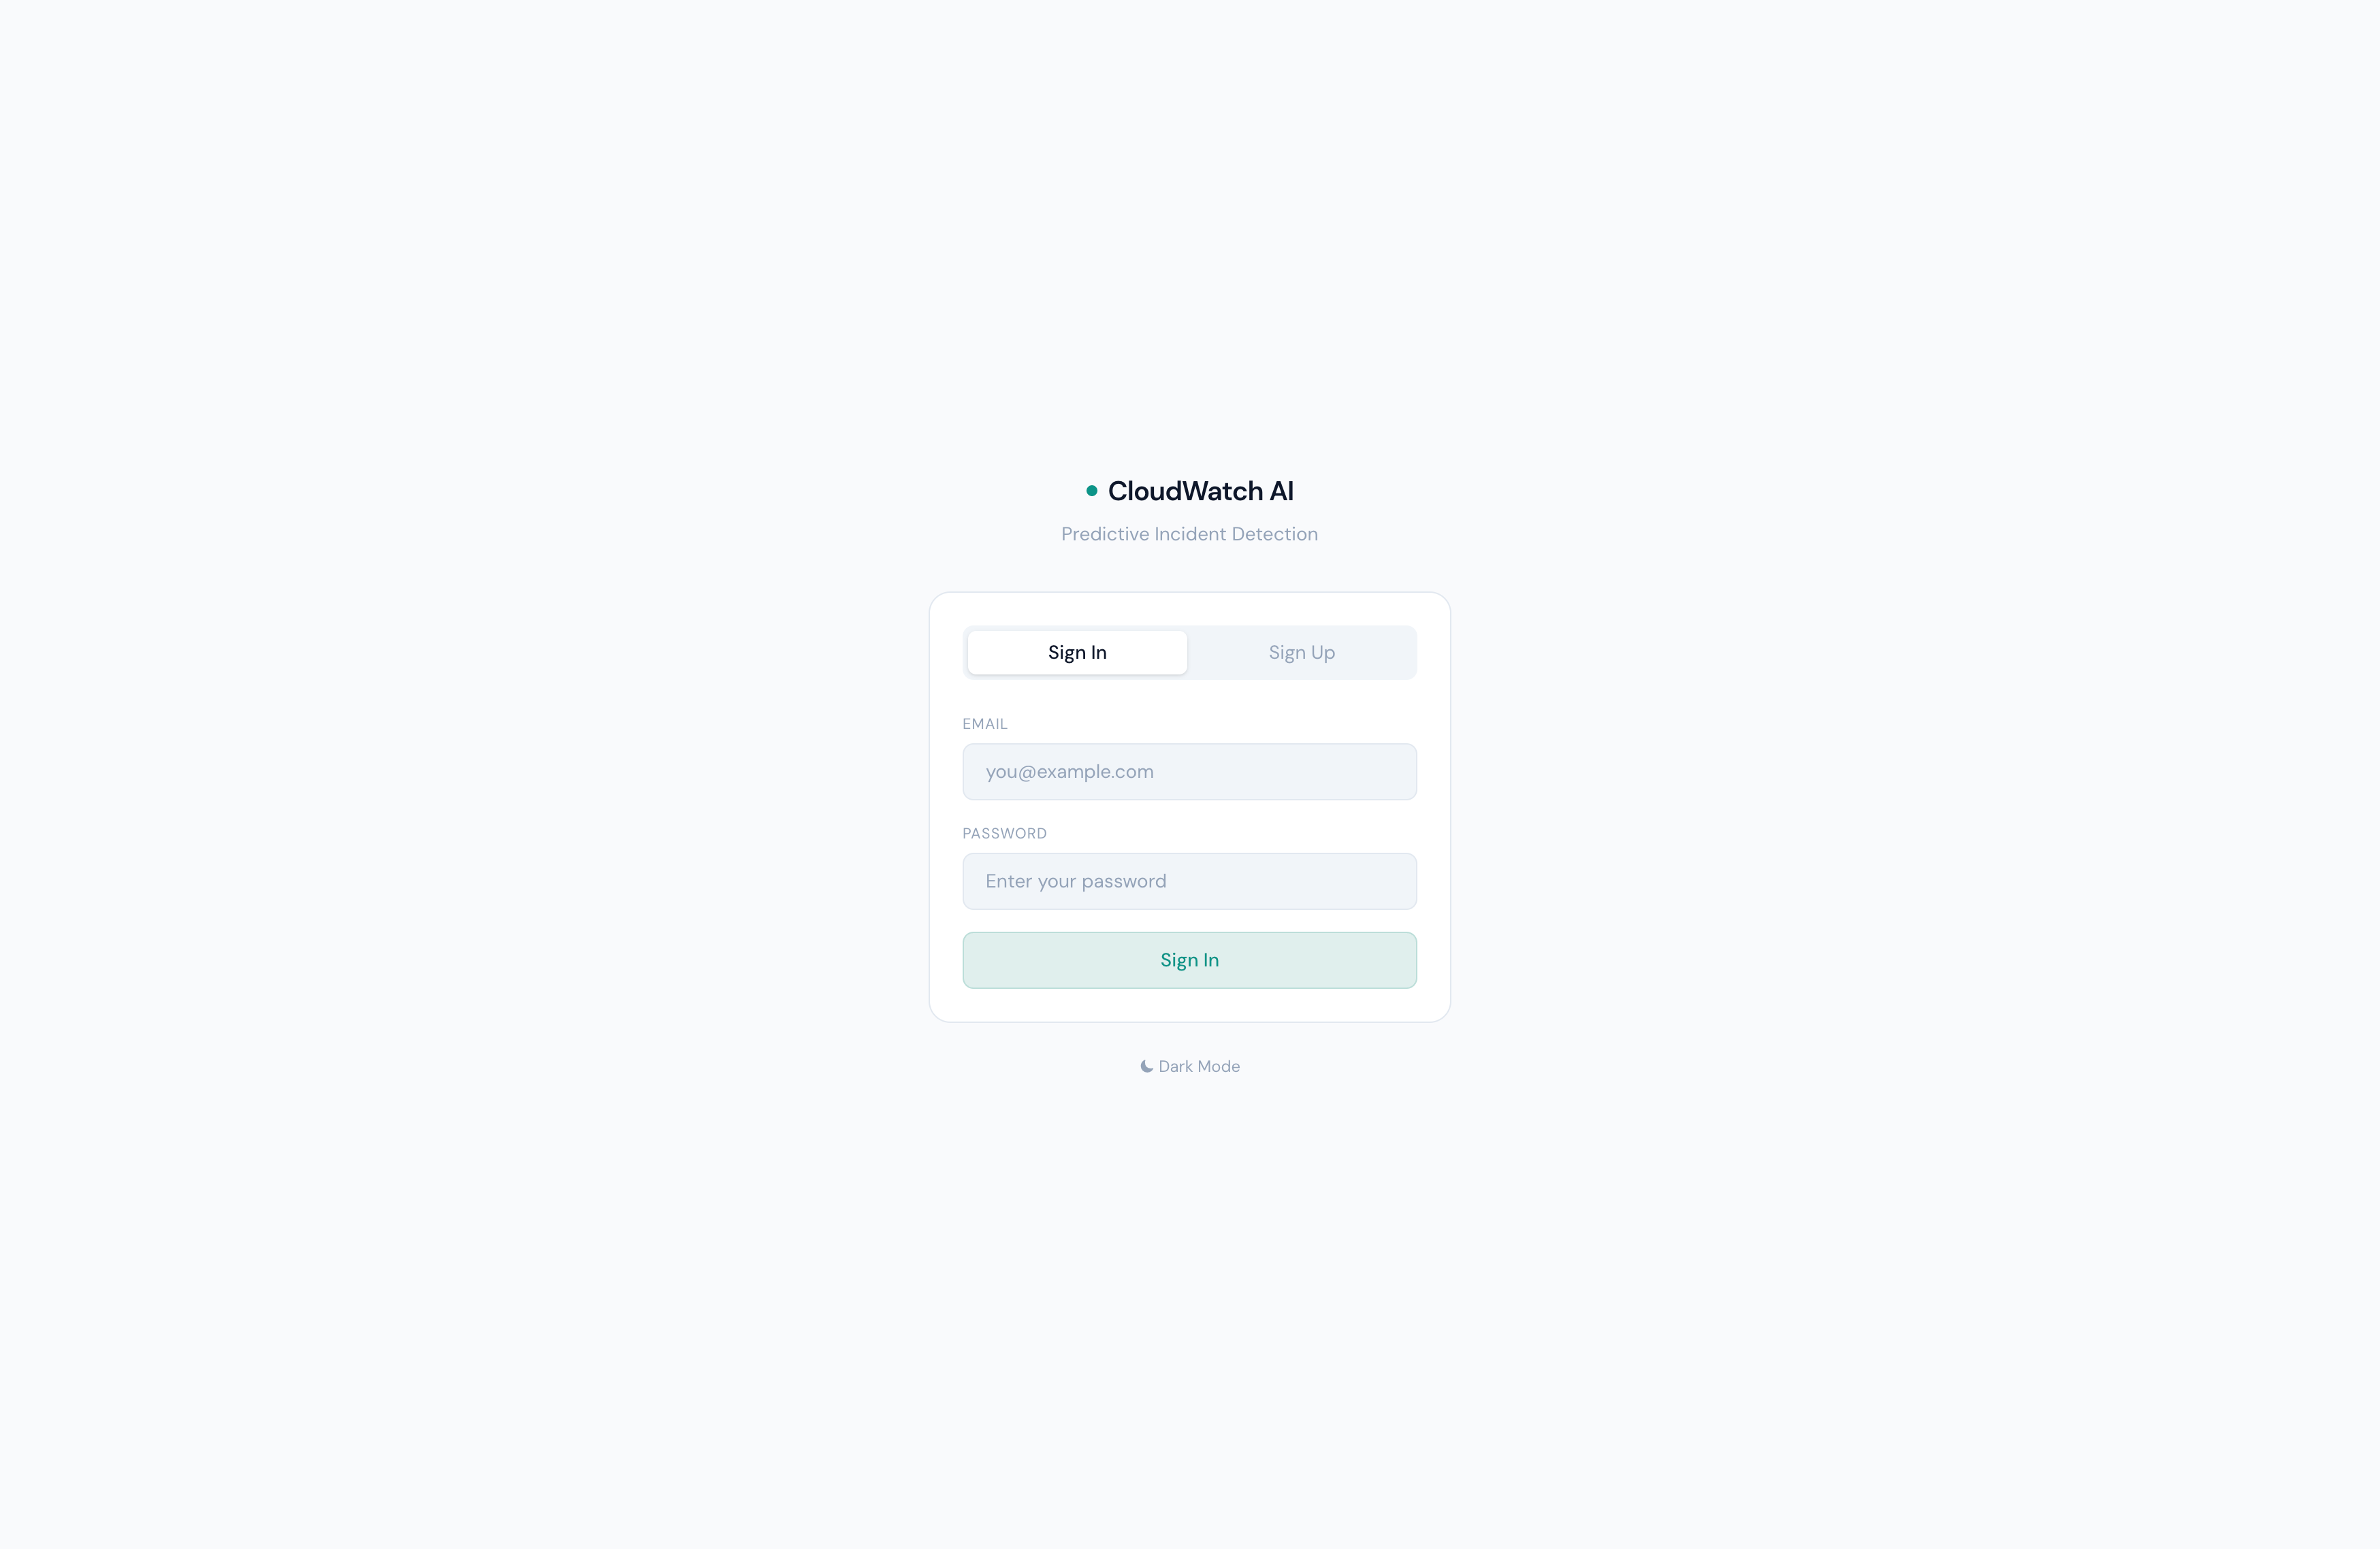
\includegraphics[width=1.0\linewidth]{images/login_page.png}
\caption{Login Page}
\label{fig:login-page}
\end{figure}

\begin{figure}[H]
\centering
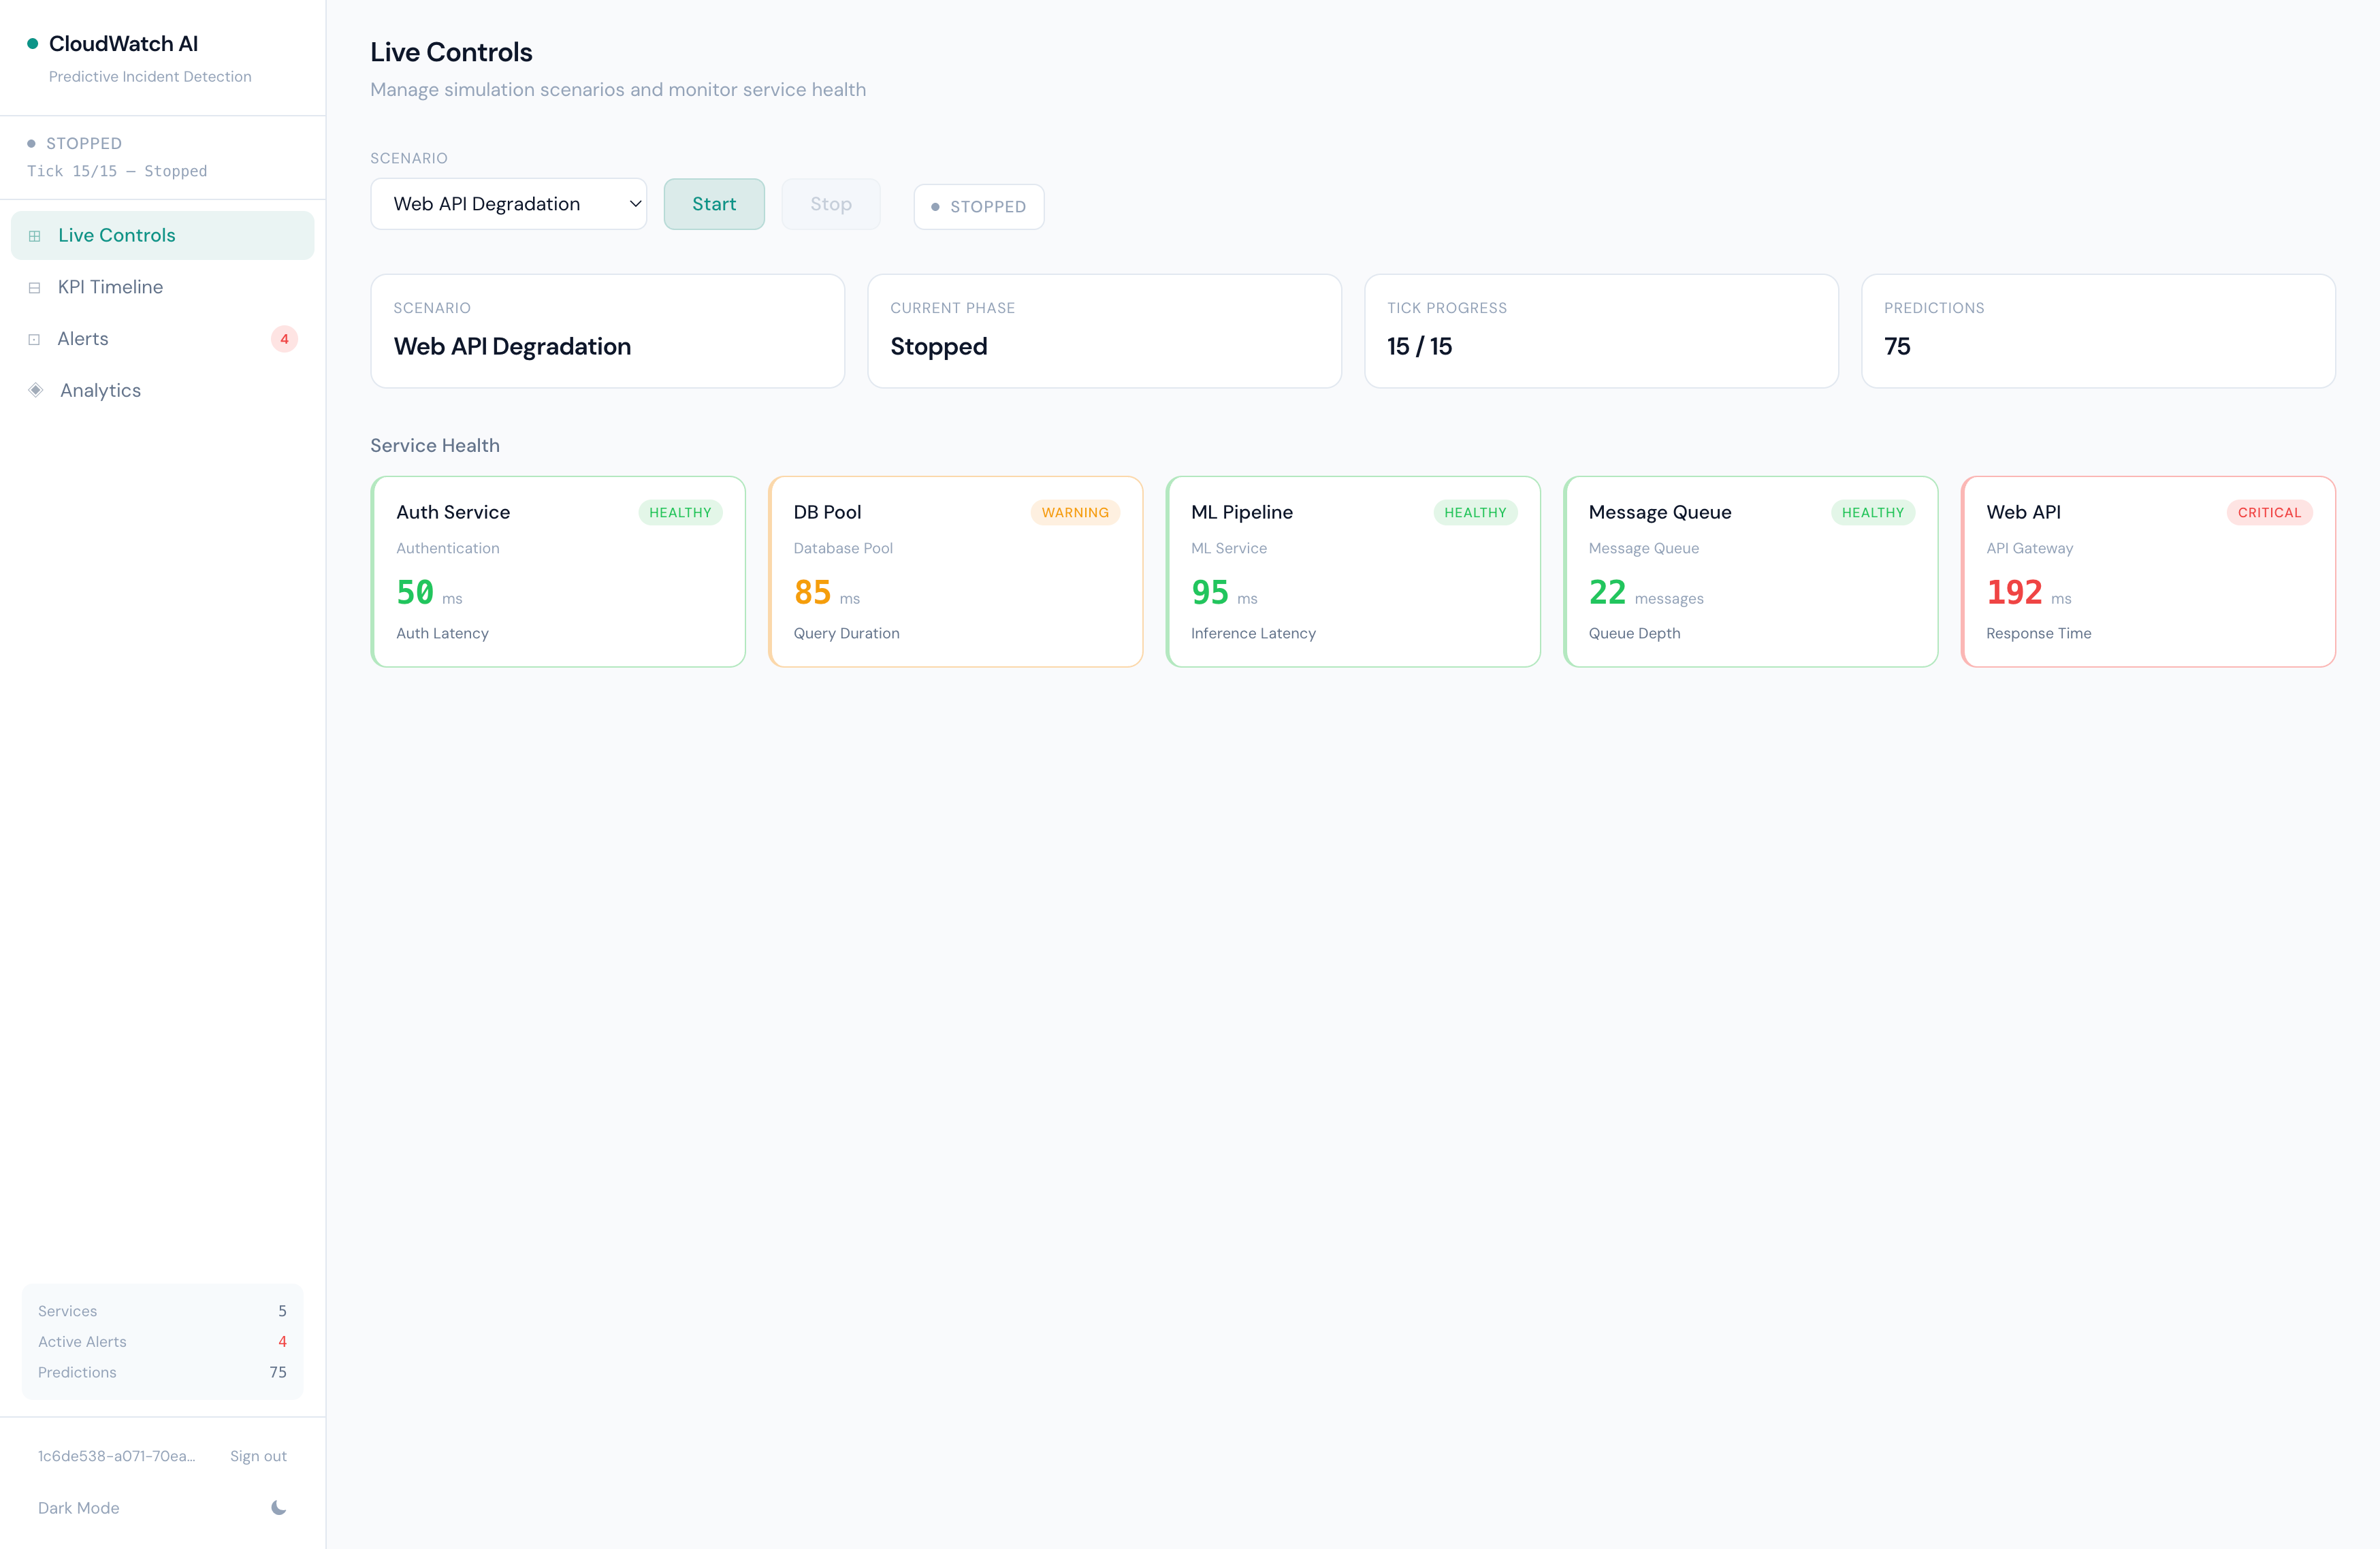
\includegraphics[width=1.0\linewidth]{images/dashboard_live_controls.png}
\caption{Dashboard -- Live Controls Page}
\label{fig:dashboard-live}
\end{figure}

\begin{figure}[H]
\centering
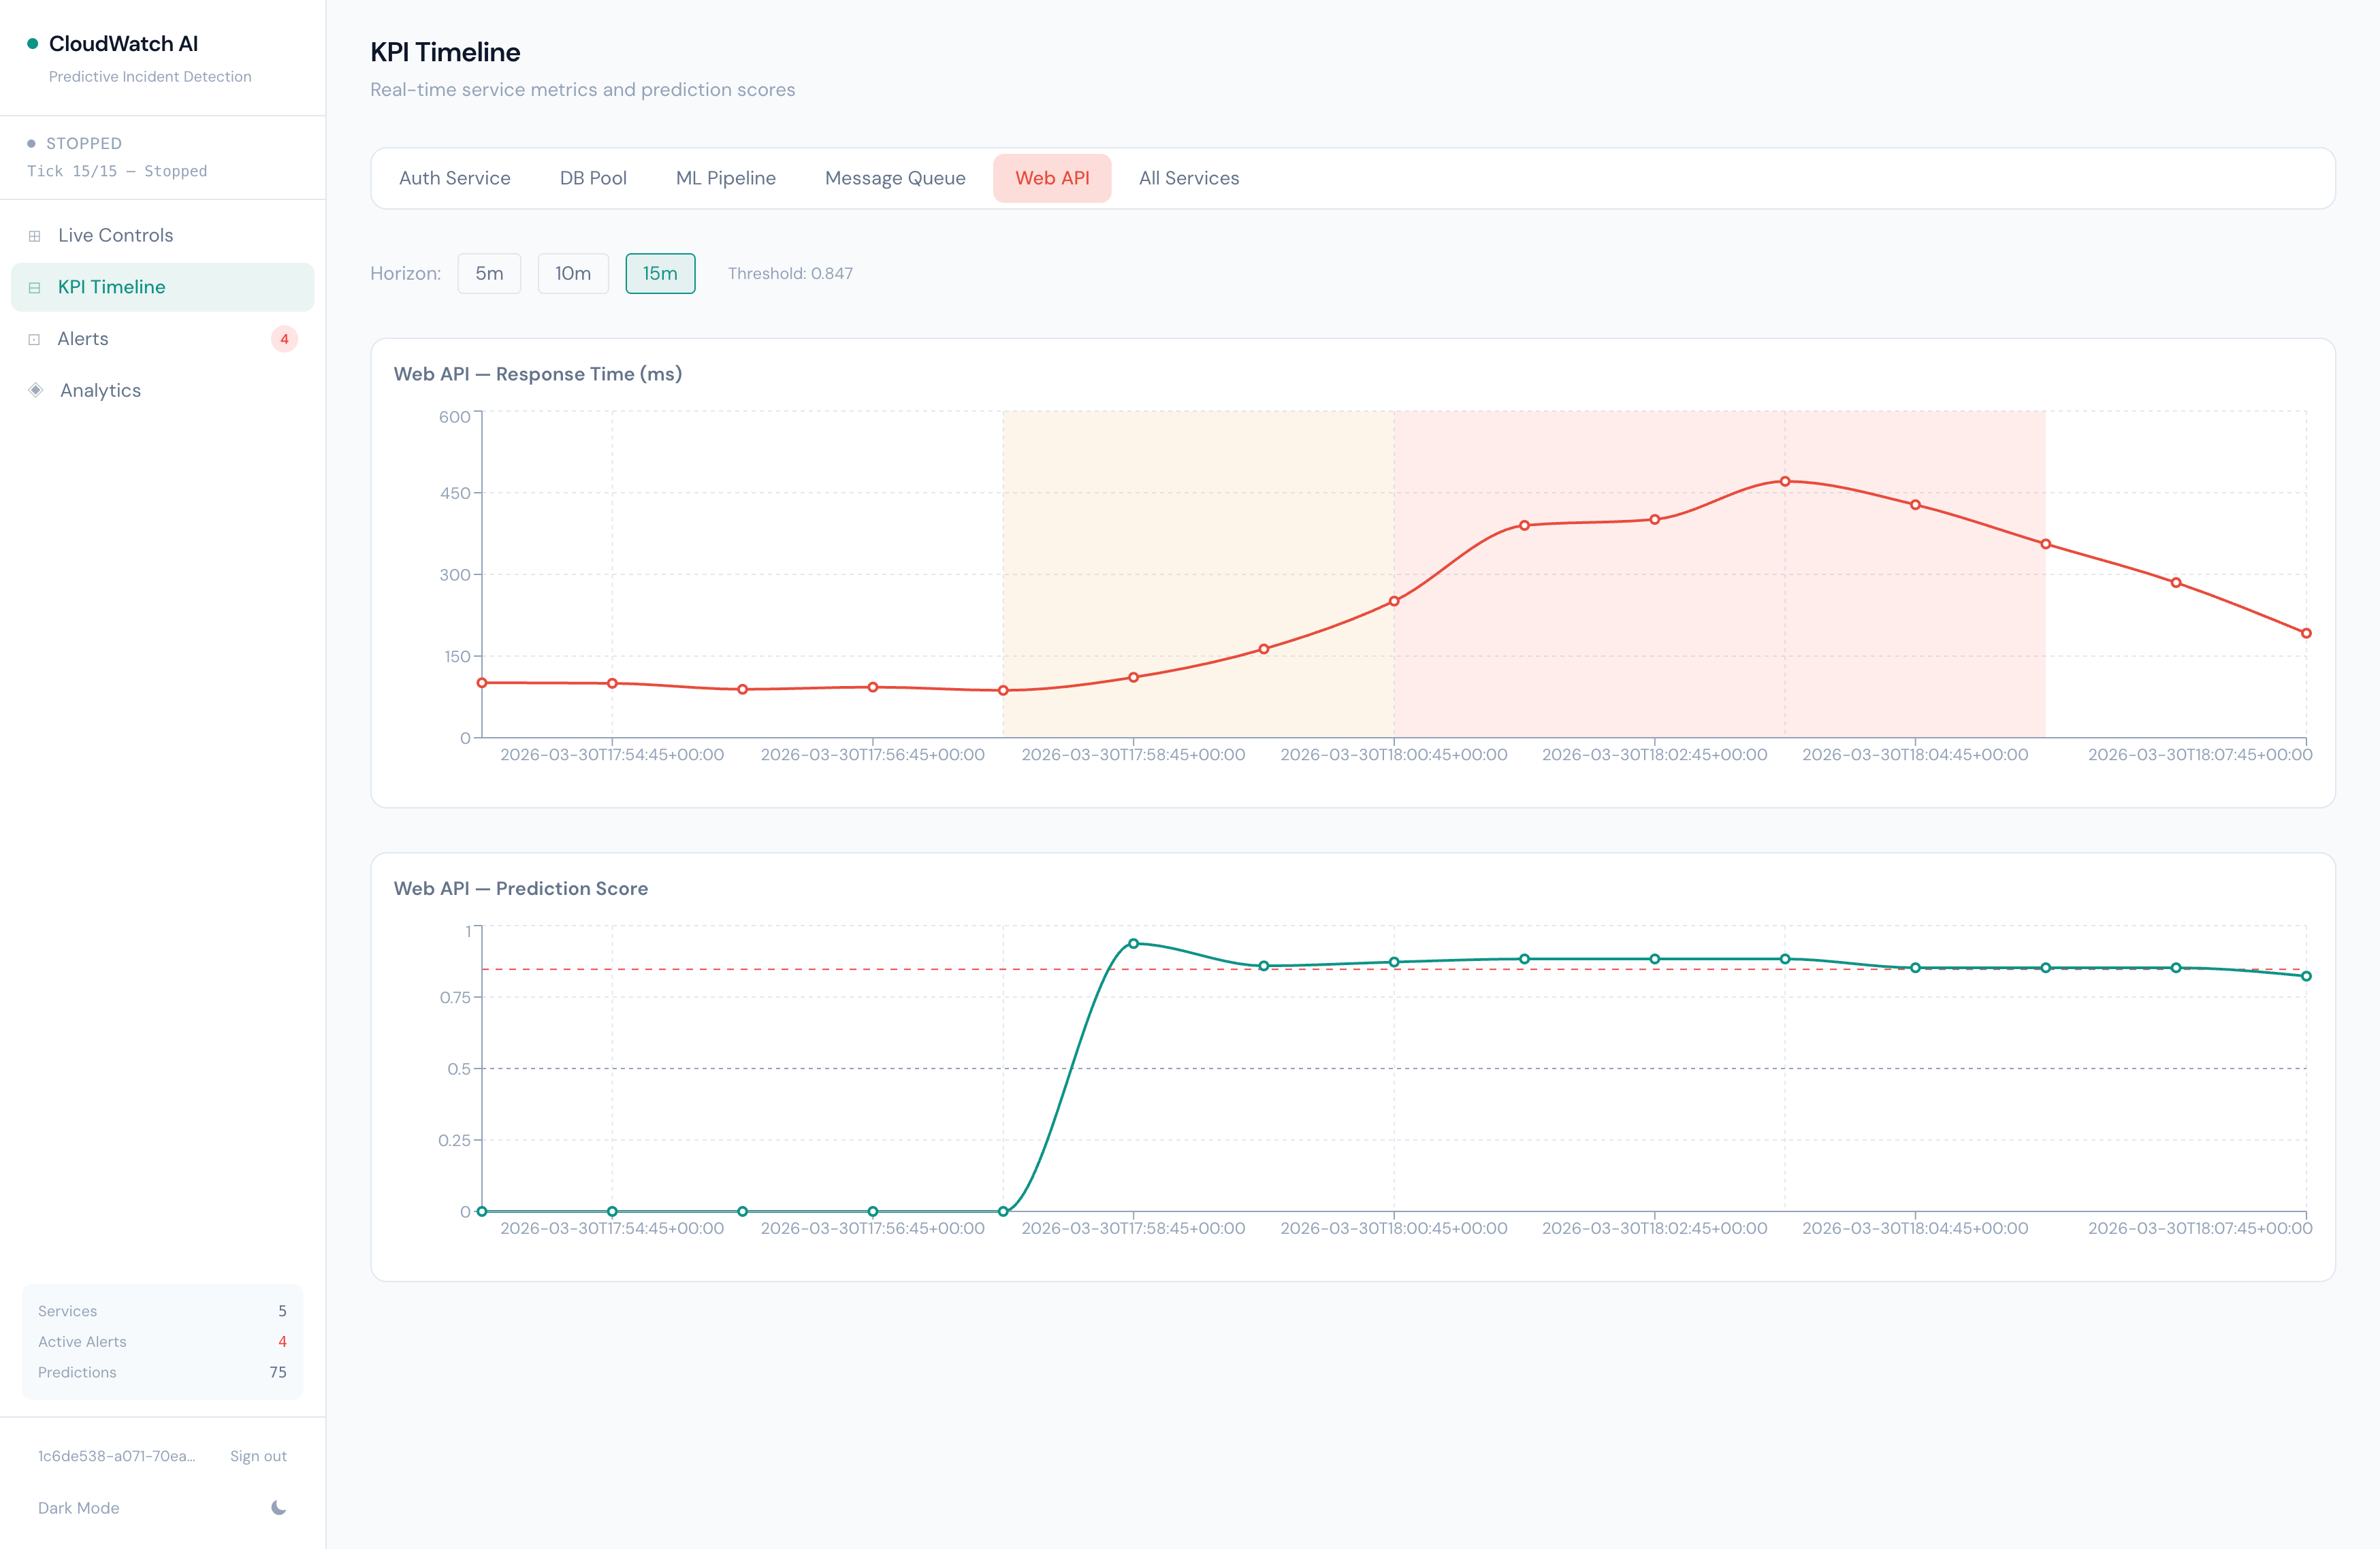
\includegraphics[width=1.0\linewidth]{images/dashboard_kpi_timeline.png}
\caption{Dashboard -- KPI Timeline Page}
\label{fig:dashboard-timeline}
\end{figure}

\begin{figure}[H]
\centering
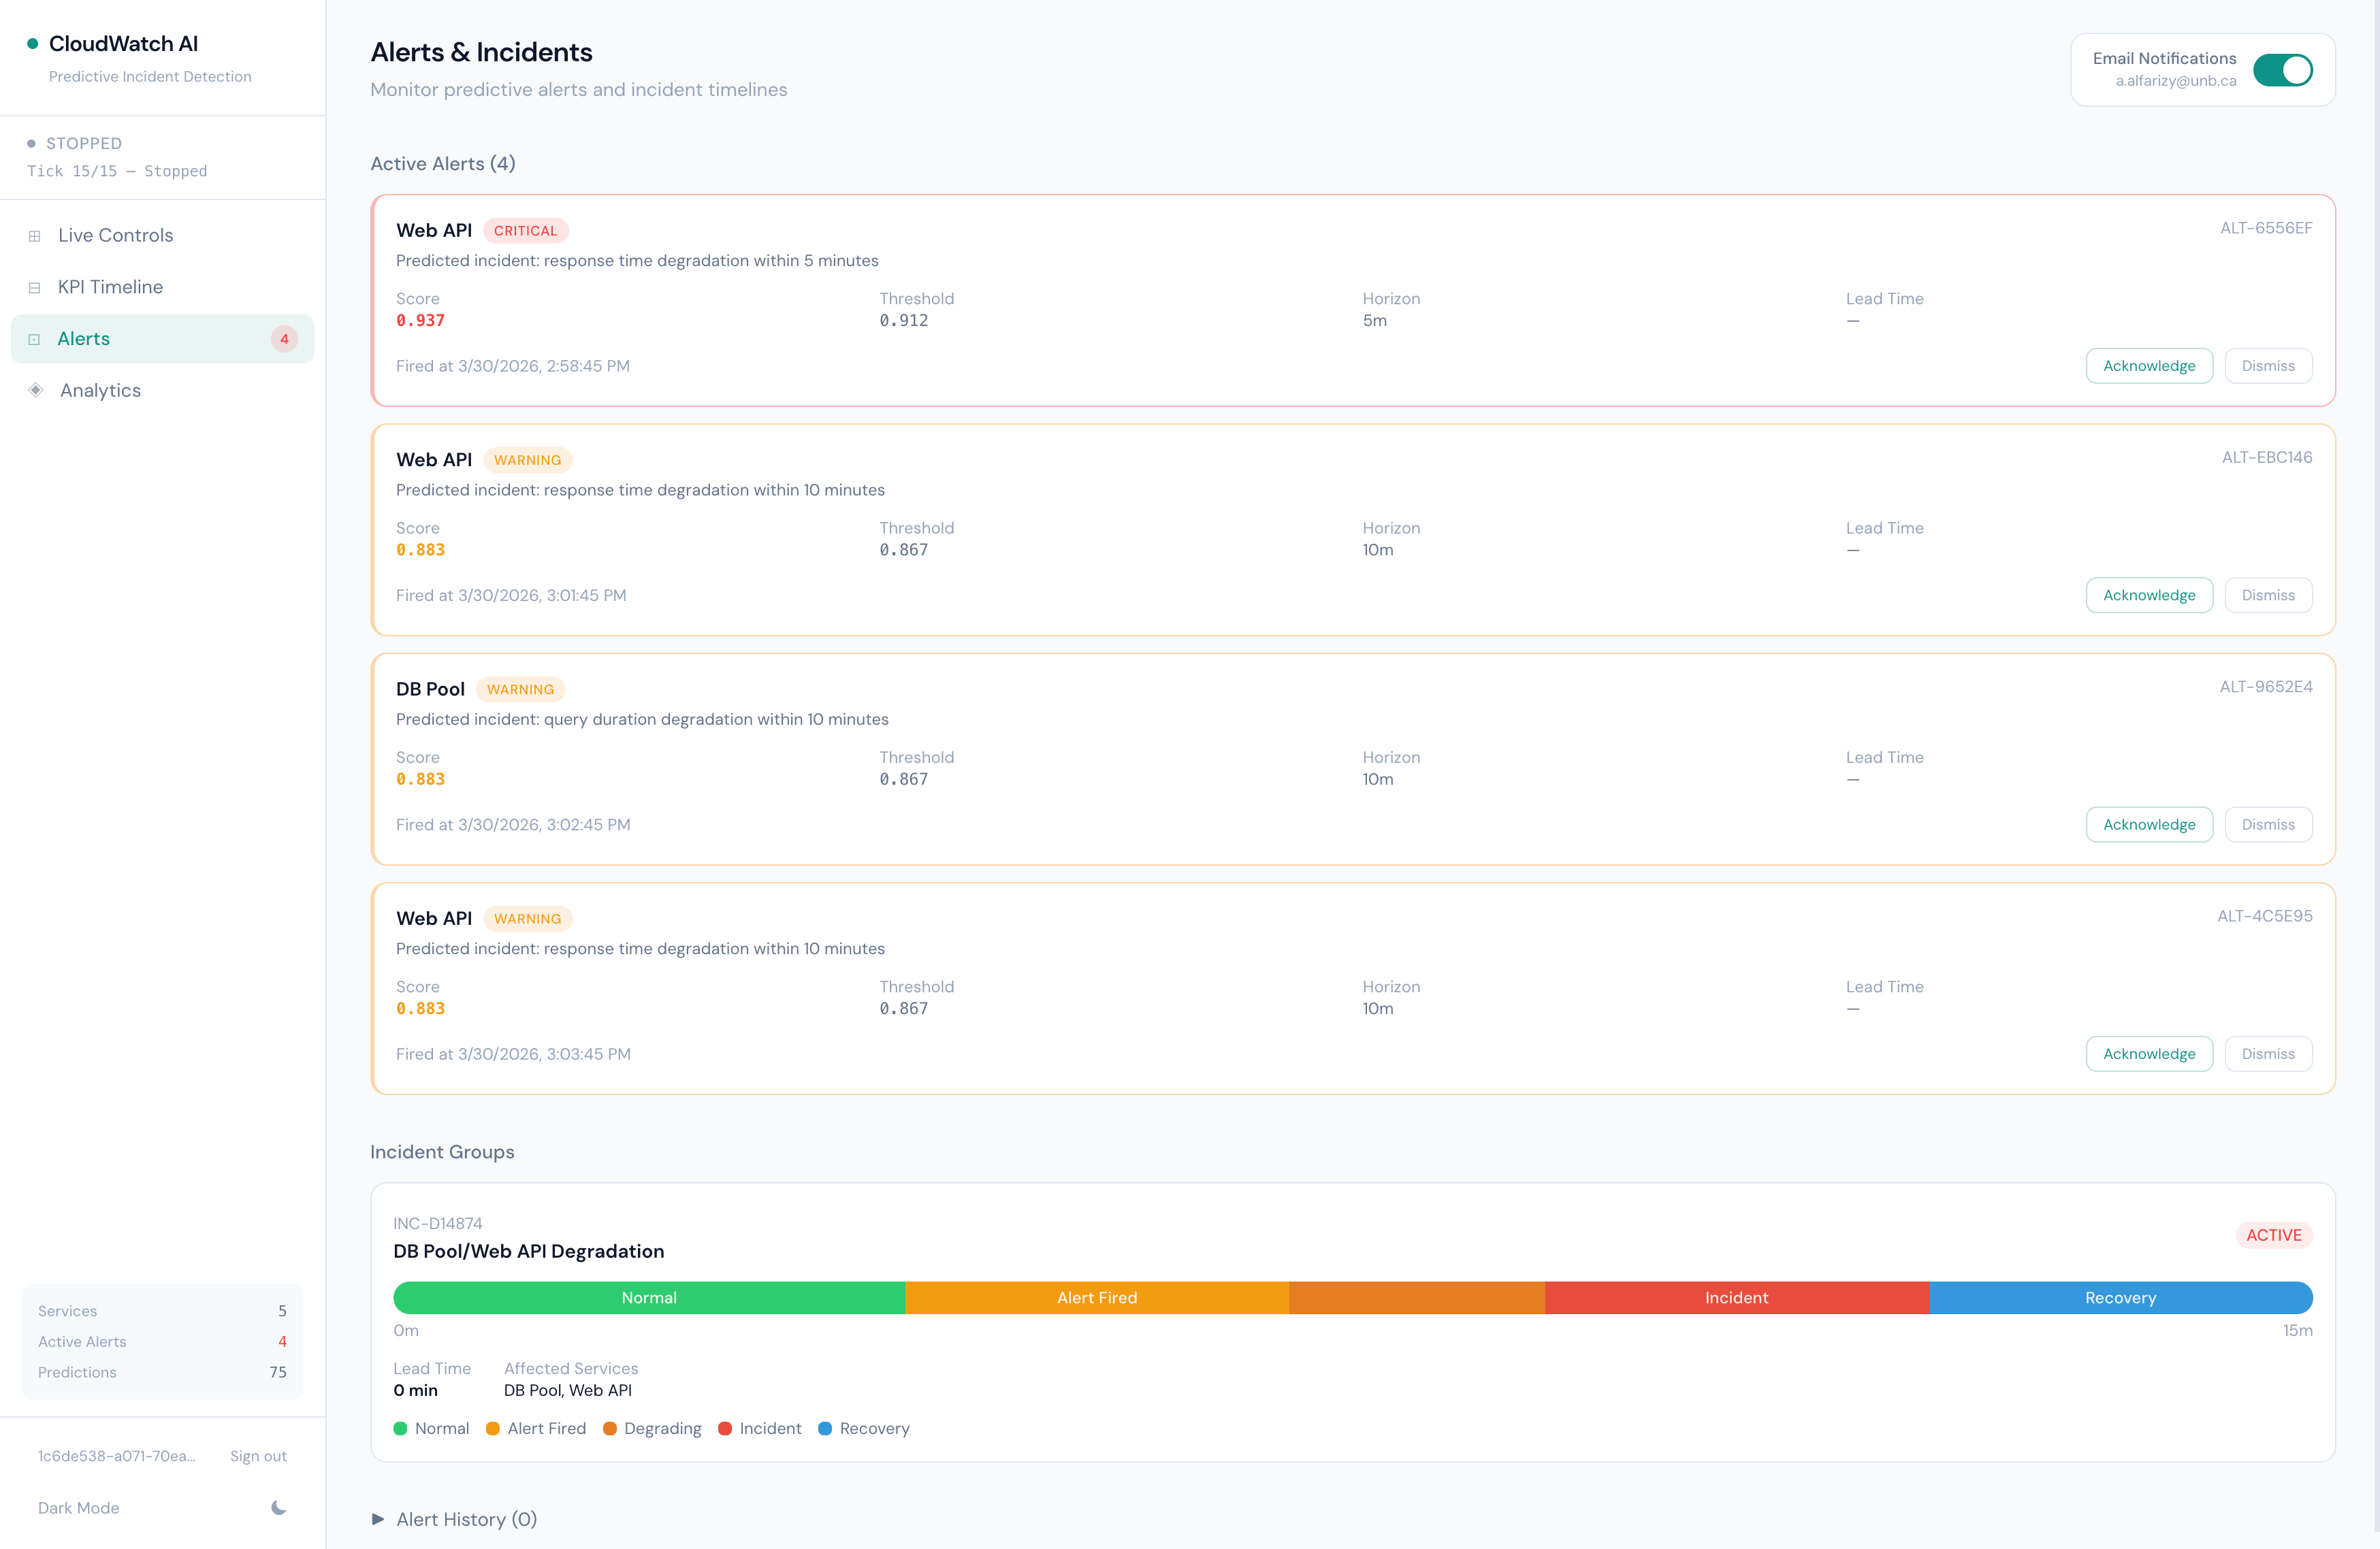
\includegraphics[width=1.0\linewidth]{images/dashboard_alerts.png}
\caption{Dashboard -- Alerts \& Incidents Page}
\label{fig:dashboard-alerts}
\end{figure}

\begin{figure}[H]
\centering
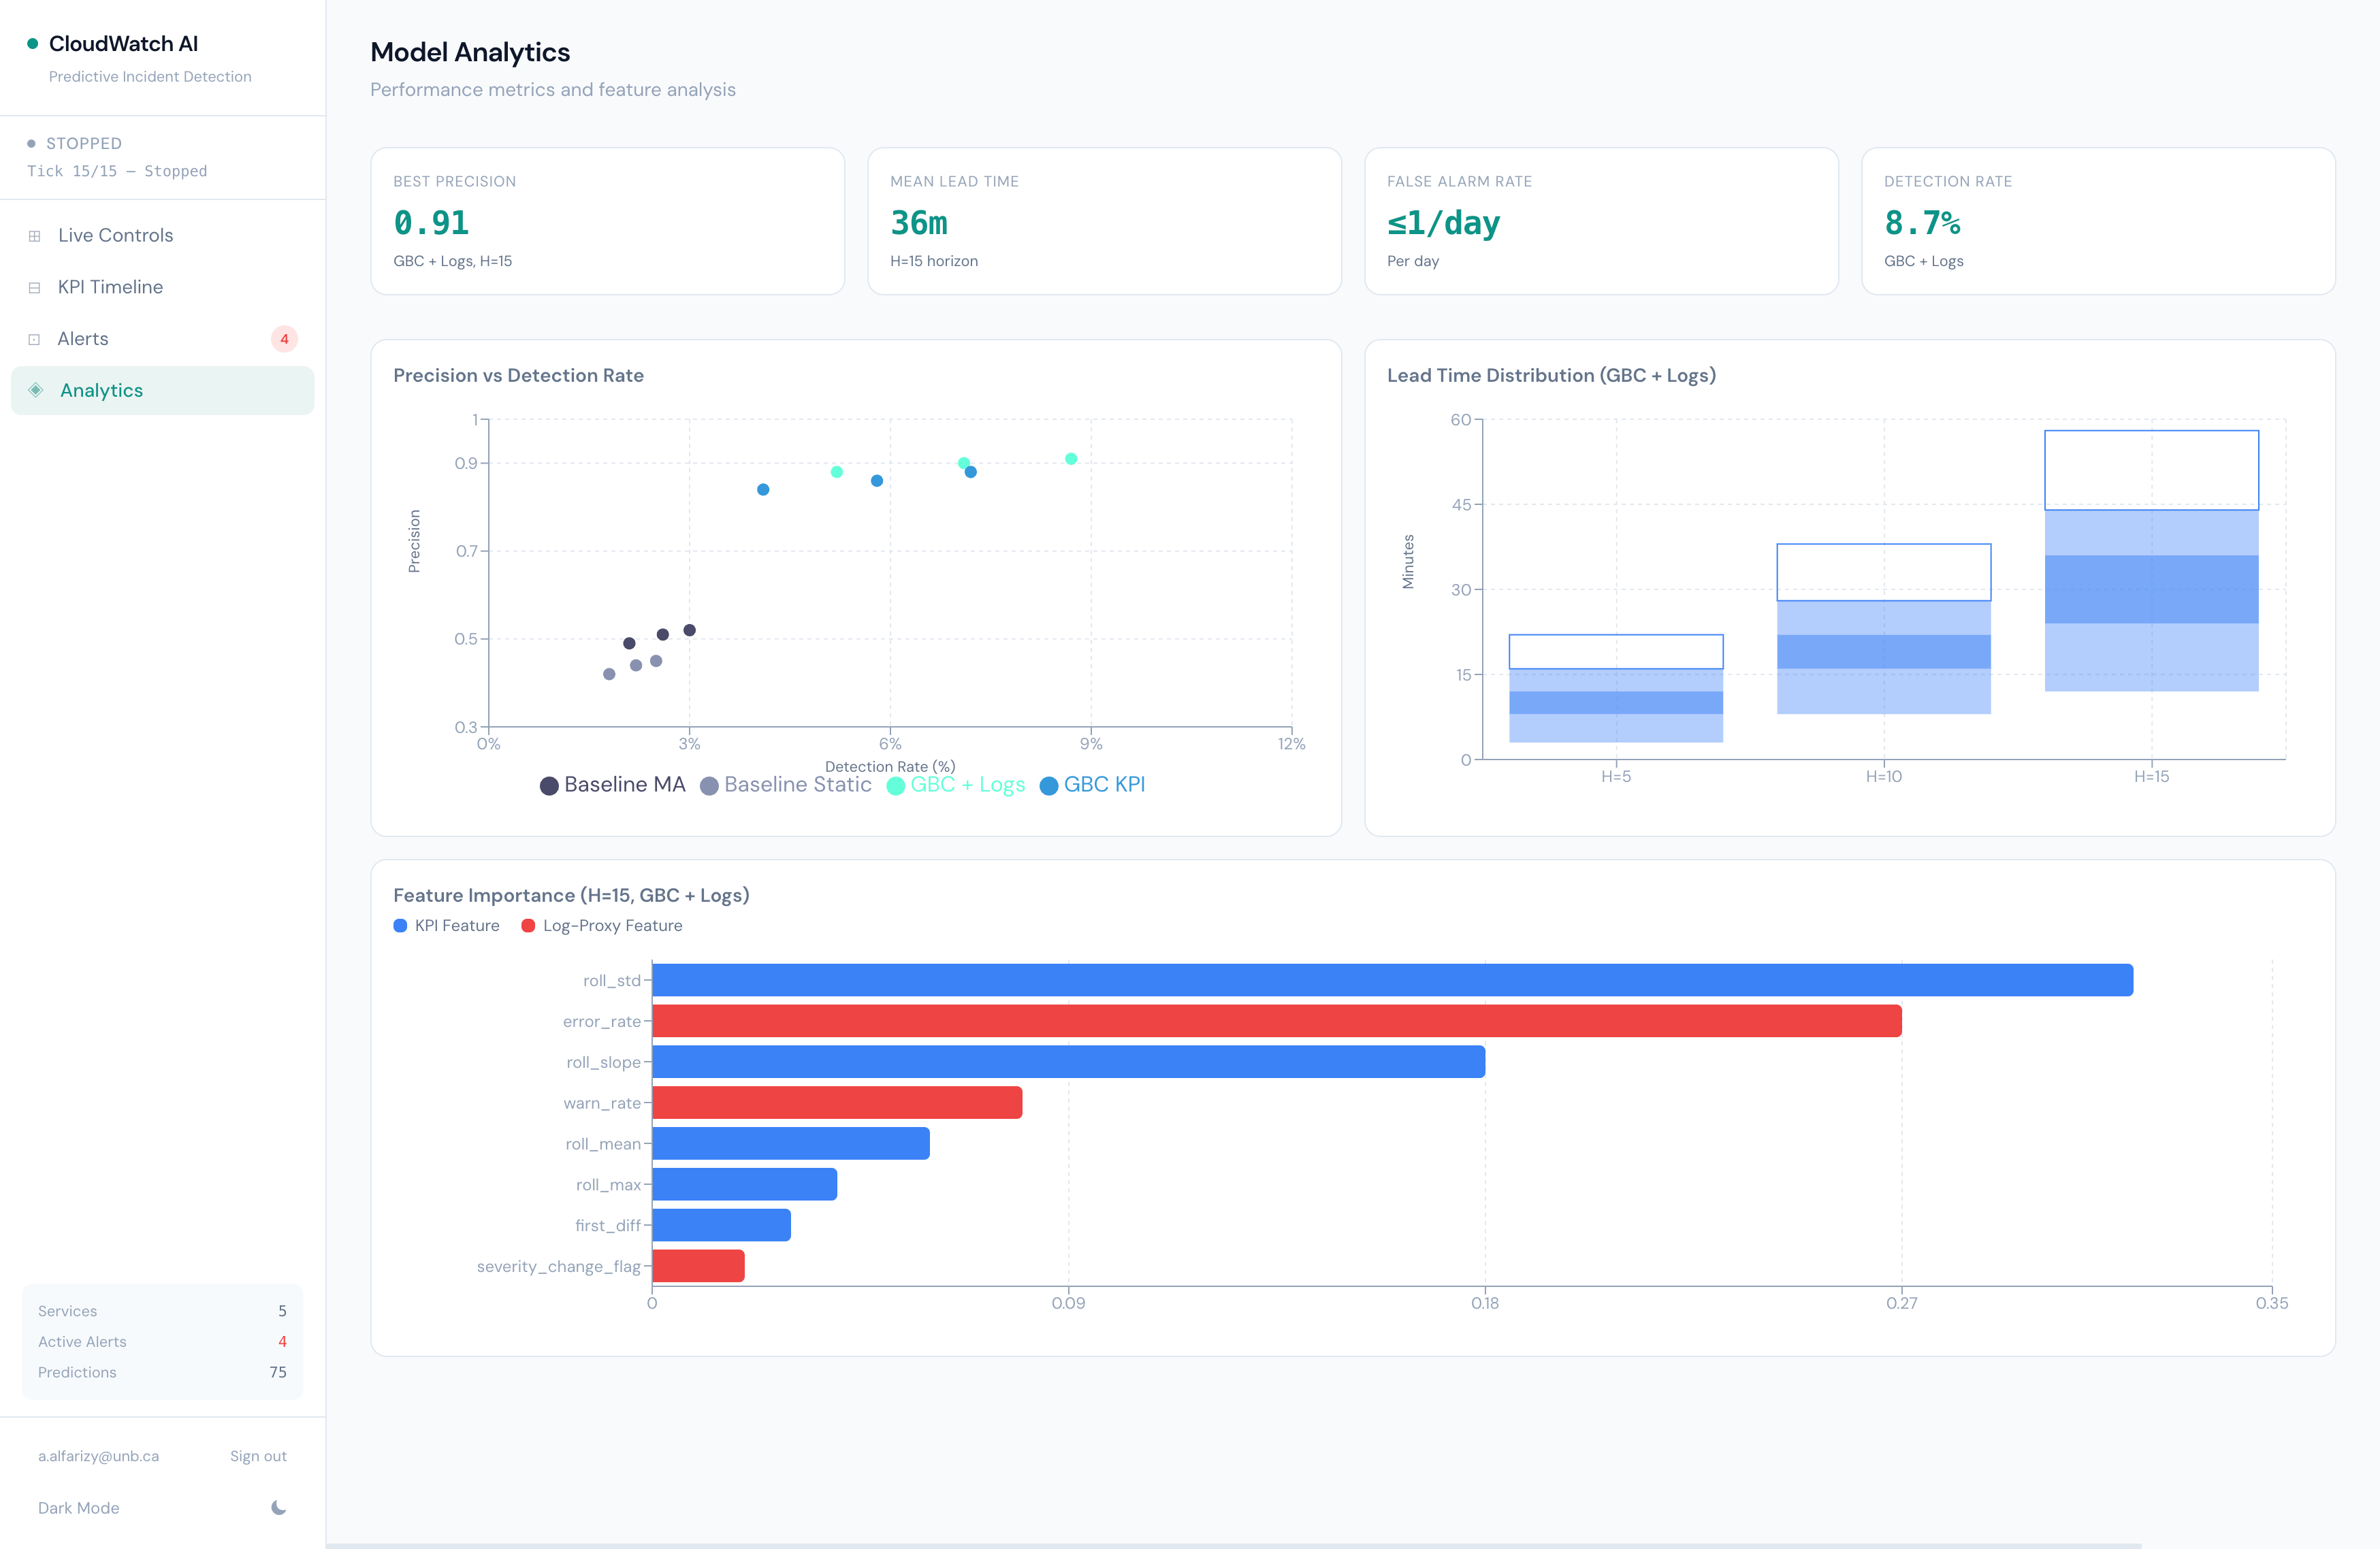
\includegraphics[width=1.0\linewidth]{images/dashboard_analytics.png}
\caption{Dashboard -- Analytics Page}
\label{fig:dashboard-analytics}
\end{figure}

\begin{figure}[H]
\centering
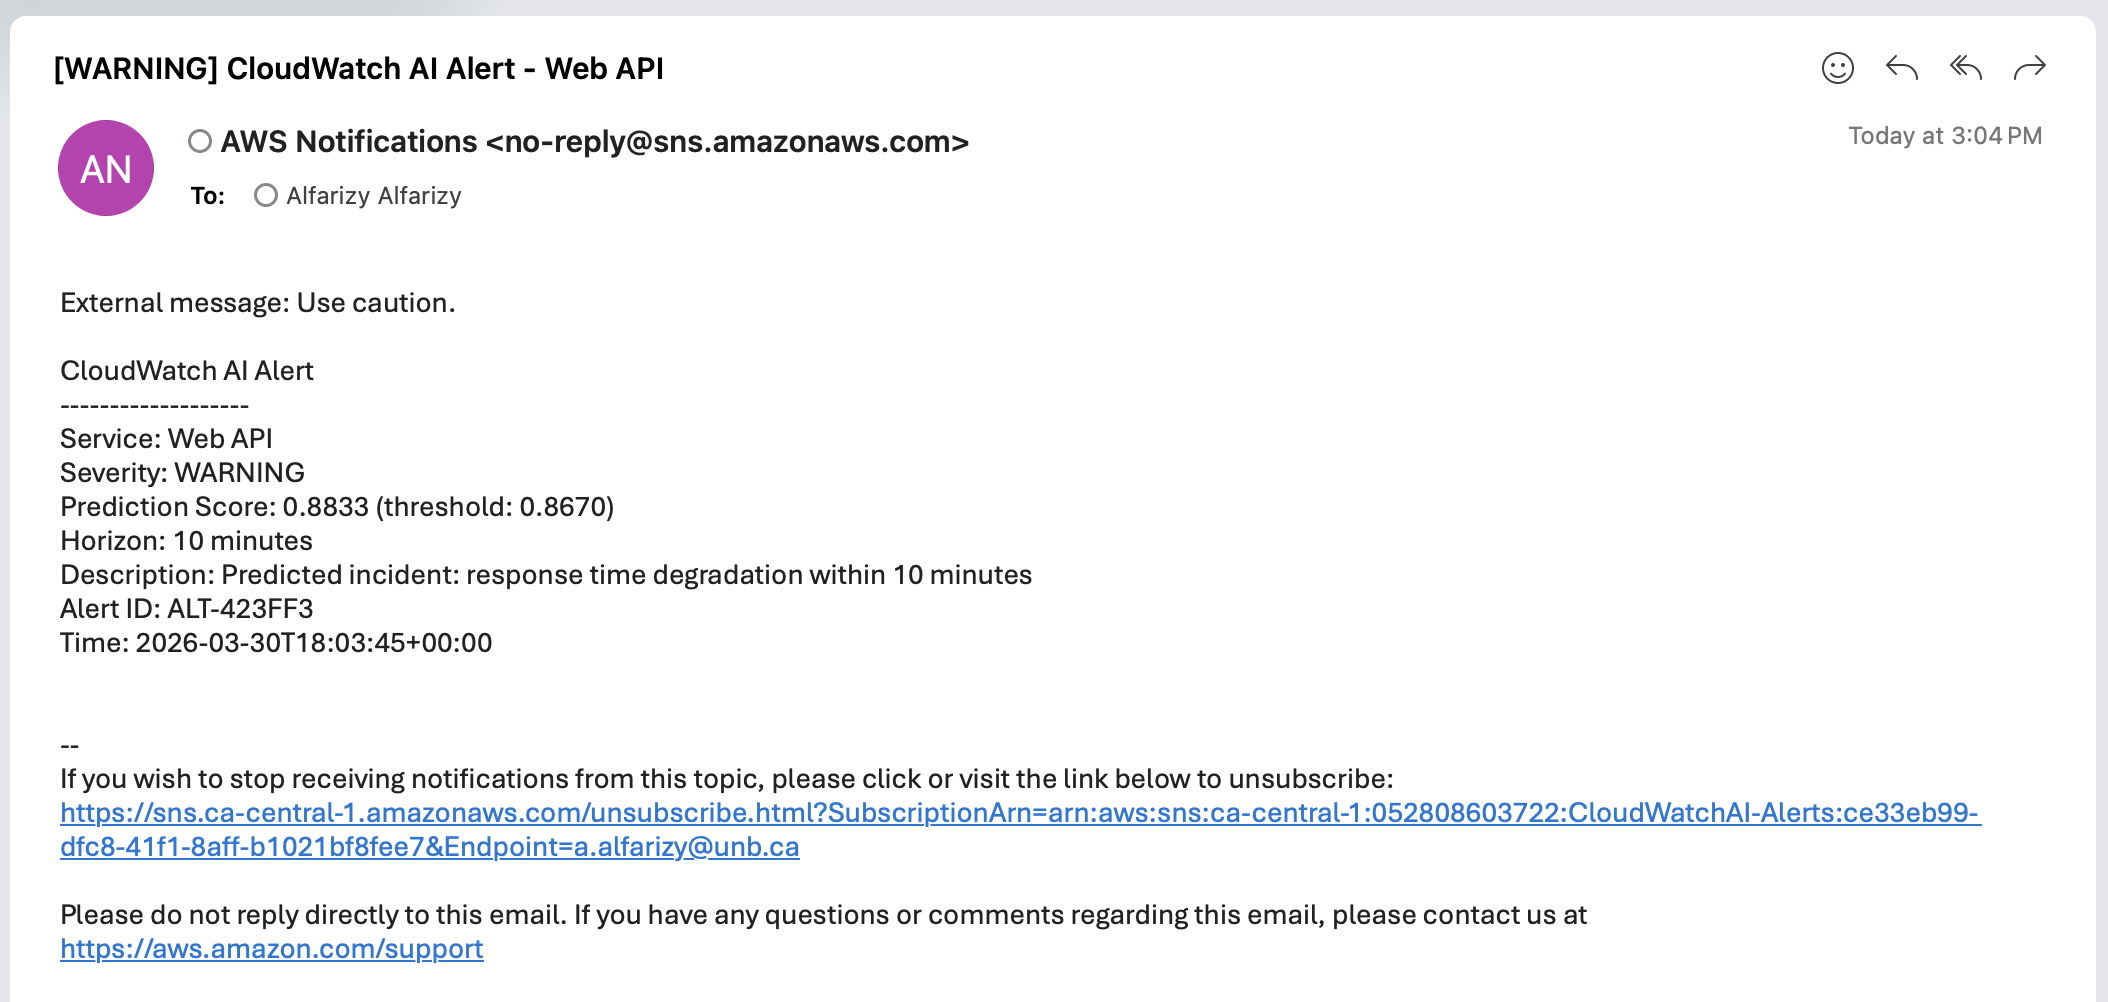
\includegraphics[width=1.0\linewidth]{images/email_notification.png}
\caption{Email Notification}
\label{fig:email-notification}
\end{figure}

% ========================
% SECTION 6: SECURITY CONFIGURATION
% ========================
\newpage
\section{Security Configuration}

\subsection{Authentication}

We handle authentication through \textbf{AWS Cognito}. The setup details are as follows:

\begin{table}[H]
\centering
\begin{tabular}{ll}
\toprule
\textbf{Property} & \textbf{Value} \\
\midrule
User Pool Name & CloudWatchAI \\
User Pool ID & \texttt{ca-central-1\_cyhaCVeUz} \\
App Client ID & \texttt{39aln1edjk2egqb9b8g82dut6j} \\
Auth Flow & SRP (Secure Remote Password) \\
Username Attribute & Email \\
Auto-Verified Attributes & Email \\
Client Secret & None (public SPA -- best practice) \\
\bottomrule
\end{tabular}
\caption{Cognito User Pool Configuration (verified from AWS)}
\label{tab:cognito-config}
\end{table}

\begin{table}[H]
\centering
\begin{tabular}{ll}
\toprule
\textbf{Requirement} & \textbf{Enforced} \\
\midrule
Minimum length & 8 characters \\
Uppercase letter & Yes \\
Lowercase letter & Yes \\
Number & Yes \\
Special character & No \\
Temporary password validity & 7 days \\
\bottomrule
\end{tabular}
\caption{Password Policy (verified from AWS)}
\label{tab:password-policy}
\end{table}

\subsection{Authorization -- JWT Authorizer}

All 19 API Gateway routes are guarded by a \textbf{JWT Authorizer} that checks tokens against our Cognito User Pool:

\begin{table}[H]
\centering
\begin{tabular}{ll}
\toprule
\textbf{Property} & \textbf{Value} \\
\midrule
Authorizer Type & JWT \\
Identity Source & \texttt{\$request.header.Authorization} \\
Issuer & \texttt{https://cognito-idp.ca-central-1.amazonaws.com/ca-central-1\_cyhaCVeUz} \\
Audience & \texttt{39aln1edjk2egqb9b8g82dut6j} \\
\bottomrule
\end{tabular}
\caption{JWT Authorizer Configuration}
\label{tab:jwt-auth}
\end{table}

On the frontend side, we wrote a \texttt{ProtectedRoute} React component that checks the Cognito session. If the user is not authenticated, it immediately redirects them to \texttt{/login}.

\subsection{Data Encryption}

\begin{table}[H]
\centering
\begin{tabular}{llll}
\toprule
\textbf{Scope} & \textbf{Service} & \textbf{Algorithm} & \textbf{Key Management} \\
\midrule
\multirow{3}{*}{At Rest} & DynamoDB (6 tables) & AES-256 & AWS-owned keys \\
 & S3 (dashboard bucket) & AES-256 (SSE-S3) & AWS-managed, BucketKey enabled \\
 & Cognito User Pool & AES-256 & AWS-managed \\
\midrule
\multirow{5}{*}{In Transit} & Browser $\leftrightarrow$ API Gateway & TLS 1.2+ & AWS-managed \\
 & Browser $\leftrightarrow$ Cognito & TLS 1.2+ & AWS-managed \\
 & API Gateway $\leftrightarrow$ Lambda & TLS 1.2+ & AWS internal \\
 & Lambda $\leftrightarrow$ DynamoDB & TLS 1.2+ & AWS SDK default \\
 & Lambda $\leftrightarrow$ S3 & TLS 1.2+ & AWS SDK default \\
\bottomrule
\end{tabular}
\caption{Encryption Configuration}
\label{tab:encryption}
\end{table}

\subsection{Access Controls}

\begin{itemize}[leftmargin=2em]
    \item Each Lambda function has its own \textbf{IAM role with least-privilege permissions} that is limited to the specific DynamoDB table ARNs and S3 bucket it actually needs to access.
    \item There is \textbf{no way to access DynamoDB directly} from outside because every query goes through a Lambda function that sits behind the authenticated API Gateway.
    \item The \textbf{S3 bucket policy} only allows public \texttt{GetObject} access (for serving the static frontend). Operations like \texttt{PutObject}, \texttt{DeleteObject}, and \texttt{ListBucket} are not exposed publicly.
    \item We have \textbf{no hardcoded secrets} anywhere in our codebase. The Cognito Client ID is public by design (this is standard practice for SPAs), and there are no API keys or credentials in source control.
\end{itemize}

\subsection{OWASP Top 10 Security Audit}

We ran a security audit against the OWASP Top 10 vulnerabilities. Table~\ref{tab:owasp} has the full results.

\begin{table}[H]
\centering
\begin{tabular}{llll}
\toprule
\textbf{\#} & \textbf{Vulnerability} & \textbf{Status} & \textbf{Notes} \\
\midrule
A01 & Broken Access Control & \cmark\ Pass & JWT on all routes; frontend guards \\
A02 & Cryptographic Failures & \cmark\ Pass & AES-256 at rest; TLS 1.2+ in transit \\
A03 & Injection & \cmark\ Pass & DynamoDB SDK uses parameterized queries \\
A04 & Insecure Design & \cmark\ Pass & Serverless; least-privilege IAM \\
A05 & Security Misconfiguration & \cmark\ Pass & Default encryption; no debug endpoints \\
A06 & Vulnerable Components & \cmark\ Pass & Current versions; no known CVEs \\
A07 & Authentication Failures & \cmark\ Pass & SRP protocol; password policy; token expiry \\
A08 & Data Integrity Failures & \cmark\ Pass & Model versioning in S3; DynamoDB Streams \\
A09 & Security Logging & \cmark\ Pass & CloudWatch Logs on all Lambda functions \\
A10 & SSRF & N/A & No user-supplied URLs processed \\
\bottomrule
\end{tabular}
\caption{OWASP Top 10 Assessment Results}
\label{tab:owasp}
\end{table}

\begin{successbox}[Security Audit Result]
\textbf{9/10 passed}, 1 N/A. \textbf{Overall risk level: Low.}

We also verified: CORS configuration, rate limiting (10K req/s burst), input validation, error handling (no stack traces leak to the client), secrets management, and DynamoDB TTL auto-cleanup.
\end{successbox}

\begin{figure}[H]
\centering
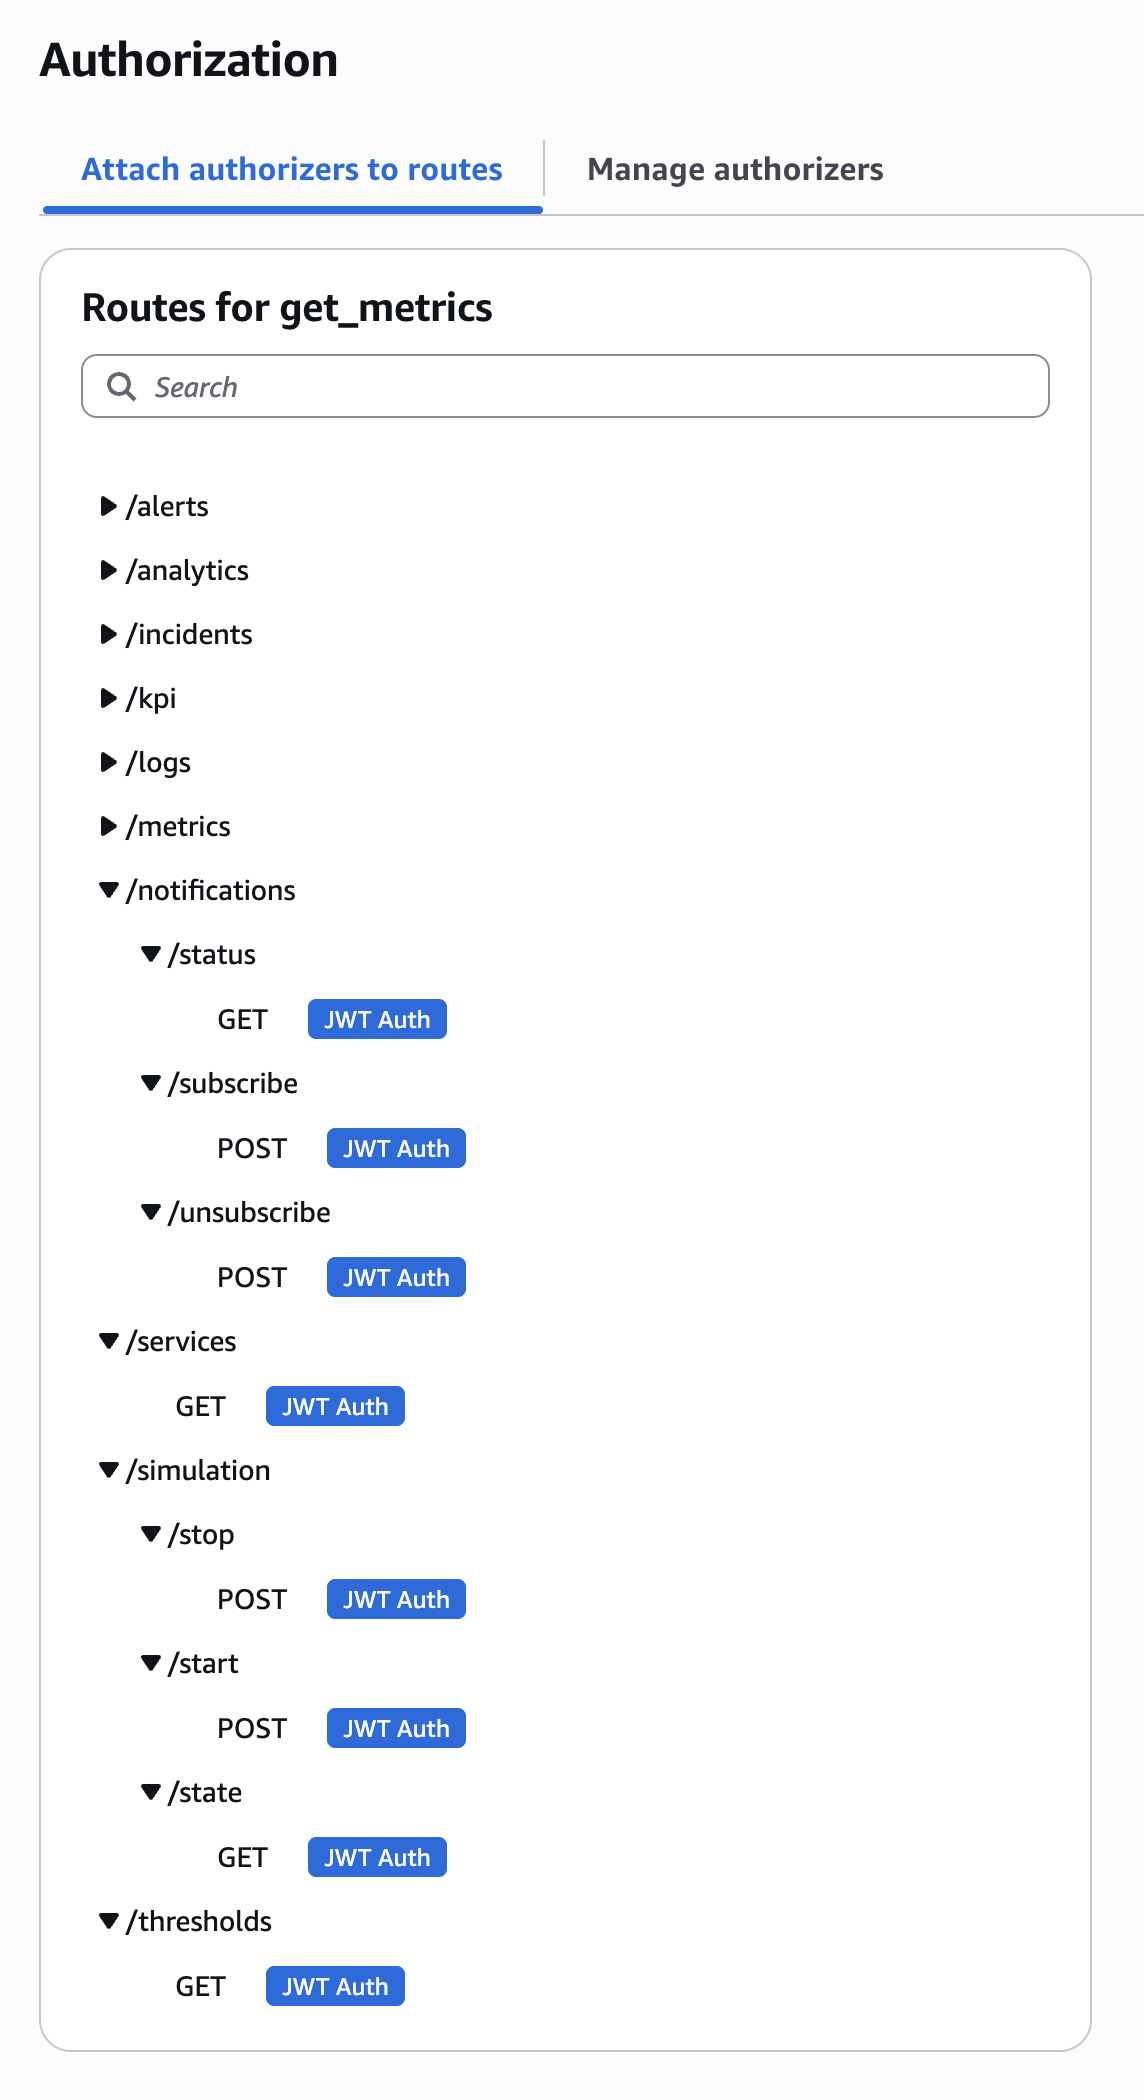
\includegraphics[width=0.6\linewidth]{images/jwt_auth.png}
\caption{API Gateway -- JWT Authorizer on all 19 routes}
\label{fig:jwt-auth}
\end{figure}

\begin{figure}[H]
\centering
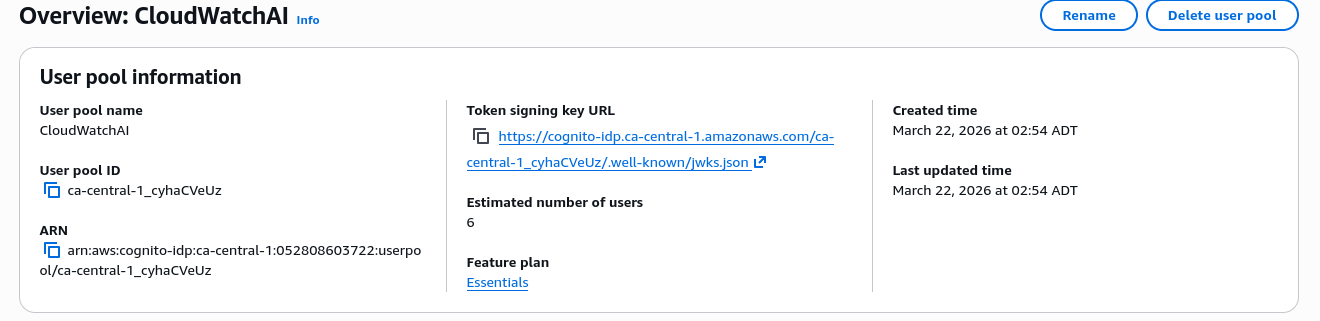
\includegraphics[width=0.9\linewidth]{images/cognito_user_pool.png}
\caption{Cognito User Pool -- Password Policy Configuration}
\label{fig:cognito-config}
\end{figure}

% ========================
% SECTION 7: INTEGRATION TESTING
% ========================
\section{Integration Testing}

\subsection{Testing Methodology}

We organized our tests into 6 categories that together cover all three system layers (frontend, backend, and database) as well as cross-cutting concerns like theming and error handling. Every test case follows a consistent format: unique ID, description, preconditions, steps, expected result, and pass/fail status.

\subsection{Test Environment}

\begin{table}[H]
\centering
\begin{tabular}{ll}
\toprule
\textbf{Component} & \textbf{Details} \\
\midrule
API Gateway & \texttt{https://p9fpx4nhh6.execute-api.ca-central-1.amazonaws.com} \\
AWS Region & \texttt{ca-central-1} \\
Cognito User Pool & \texttt{ca-central-1\_cyhaCVeUz} \\
S3 Production URL & \texttt{cloud-project-dashboard1.s3-website.ca-central-1.amazonaws.com} \\
Frontend Dev Server & \texttt{http://localhost:5173} \\
Browser & Chrome 133+ / Safari 18+ \\
Test Date & March 22, 2026 \\
\bottomrule
\end{tabular}
\caption{Test Environment}
\label{tab:test-env}
\end{table}

\subsection{Test Results Summary}

\begin{table}[H]
\centering
\begin{tabular}{lccc}
\toprule
\textbf{Category} & \textbf{Total} & \textbf{Pass} & \textbf{Fail} \\
\midrule
Authentication (CLI) & 5 & 5 & 0 \\
API Endpoints & 14 & 14 & 0 \\
Simulation Lifecycle & 5 & 5 & 0 \\
Database Verification & 5 & 5 & 0 \\
Production Deployment (CLI) & 3 & 3 & 0 \\
\midrule
\textbf{Subtotal (Automated)} & \textbf{32} & \textbf{32} & \textbf{0} \\
\midrule
Authentication (Browser) & 4 & -- & -- \\
Frontend Integration & 17 & -- & -- \\
Cross-Cutting (Theme, Error, etc.) & 7 & -- & -- \\
Production Deployment (Browser) & 1 & -- & -- \\
\midrule
\textbf{Subtotal (Manual)} & \textbf{29} & \multicolumn{2}{c}{\textit{Documented}} \\
\midrule
\textbf{Grand Total} & \textbf{61} & & \\
\bottomrule
\end{tabular}
\caption{Integration Test Results}
\label{tab:test-results}
\end{table}

\subsection{Key Test Cases and Results}

\subsubsection{Authentication Tests (5/5 Passed)}

\begin{itemize}[leftmargin=2em]
    \item \textbf{AUTH-01: User Registration} -- We confirmed that Cognito creates the user in an unconfirmed state and sends out an email verification code. \cmark
    \item \textbf{AUTH-02: Email Verification} -- Entering the 6-digit code confirms the account, and the user is auto-signed in. \cmark
    \item \textbf{AUTH-03: User Sign In} -- The SRP handshake completes and returns JWT tokens; the browser redirects to the dashboard. \cmark
    \item \textbf{AUTH-04: Session Persistence} -- After refreshing the page, the session is still active thanks to the Cognito SDK. \cmark
    \item \textbf{AUTH-05: Sign Out} -- Clicking sign out clears the session and takes the user back to the login page. \cmark
\end{itemize}

\subsubsection{API Endpoint Tests (14/14 Passed)}

All 14 testable API endpoints returned the correct JSON schemas with the expected data types. Here is a quick sample of what we checked:

\begin{lstlisting}[language=bash, caption={API test output: GET /services returns 5 services with correct schema}]
$ curl -s "$BASE/services" -H "Authorization: $TOKEN" | jq 'length'
5

$ curl -s "$BASE/kpi/web-api-001" -H "Authorization: $TOKEN" | jq '.[0]'
{
  "minute": 0,
  "timestamp": "2026-03-22T04:45:01+00:00",
  "value": 87,
  "predictionScore": 0
}
\end{lstlisting}

\subsubsection{Simulation Lifecycle Tests (5/5 Passed)}

\begin{itemize}[leftmargin=2em]
    \item \textbf{SIM-01: Start Simulation} -- Sending \texttt{POST /simulation/start} kicked off data generation, and we verified that EventBridge triggered the simulator Lambda. \cmark
    \item \textbf{SIM-02: Data Pipeline Execution} -- We confirmed the full chain ran end to end: Simulator $\rightarrow$ KPIMetrics $\rightarrow$ Feature Engineering $\rightarrow$ FeatureStore $\rightarrow$ Inference $\rightarrow$ Alerts. \cmark
    \item \textbf{SIM-03: Alert Generation} -- Alerts appeared whenever the prediction score crossed the threshold, and the severity was classified correctly. \cmark
    \item \textbf{SIM-04: Incident Grouping} -- When multiple alerts fired within a 5-minute window, they were grouped into an incident record that included the list of affected services. \cmark
    \item \textbf{SIM-05: Stop Simulation} -- After stopping, no further data was generated. \cmark
\end{itemize}

\subsubsection{Database Verification Tests (5/5 Passed)}

\begin{itemize}[leftmargin=2em]
    \item \textbf{DB-01: Table Existence and Schema} -- All 6 tables are present with the right key schemas, as we confirmed by running \texttt{aws dynamodb describe-table} on each. \cmark
    \item \textbf{DB-02: DynamoDB Streams Enabled} -- Streams are active on both KPIMetrics and FeatureStore, with the \texttt{NEW\_IMAGE} view type. \cmark
    \item \textbf{DB-03: KPI Record Integrity} -- Records contain every required field, including the service-specific metrics unique to each service type. \cmark
    \item \textbf{DB-04: Alert Record Integrity} -- Alert records have all the fields that the frontend needs to render them. \cmark
    \item \textbf{DB-05: S3 Model Files} -- All 5 model files are present in S3 and accessible: 3 model pickle files plus the thresholds and feature importances JSON files. \cmark
\end{itemize}

\subsubsection{Production Deployment Tests (3/3 Passed)}

\begin{itemize}[leftmargin=2em]
    \item \textbf{PROD-01: S3 Static Hosting} -- The dashboard loads at the S3 website endpoint, and all CSS/JS assets come through correctly. \cmark
    \item \textbf{PROD-02: SPA Routing} -- Navigating directly to \texttt{/timeline} or \texttt{/alerts} in the browser works, thanks to the S3 error document configuration. \cmark
    \item \textbf{PROD-04: ML Models in S3} -- The model files are accessible, and the inference Lambda can load them without issues. \cmark
\end{itemize}

\subsection{Manual Test Documentation}

We documented 29 additional test cases that require a real browser to run. These cover:

\begin{itemize}[leftmargin=2em]
    \item \textbf{4 authentication tests}: route protection, token injection, invalid credential handling, and password policy enforcement
    \item \textbf{17 frontend integration tests}: service health card rendering, simulation controls, KPI timeline navigation, horizon toggle behavior, alert acknowledge/dismiss flow, incident timeline display, analytics chart rendering, and sidebar functionality
    \item \textbf{7 cross-cutting tests}: dark/light theme toggle, theme persistence across page reloads, loading state indicators, error handling when offline, and 401 response handling
    \item \textbf{1 production test}: confirming that the production deployment talks to the API Gateway endpoint directly (without the dev proxy)
\end{itemize}

% ========================
% SECTION 8: CHALLENGES AND SOLUTIONS
% ========================
\section{Challenges and Solutions}

\begin{xltabular}{\textwidth}{>{\bfseries}p{3.5cm}XX}
\toprule
\textbf{Challenge} & \textbf{Problem} & \textbf{Solution} \\
\midrule
\endfirsthead

\toprule
\textbf{Challenge} & \textbf{Problem} & \textbf{Solution} \\
\midrule
\endhead

\bottomrule
\caption{Implementation Challenges and Solutions} \\
\label{tab:challenges}
\endfoot

Lambda Package Size & scikit-learn, numpy, scipy, and pandas together blow past Lambda's 250 MB deployment limit & We packaged the inference Lambda as a Docker container image and pushed it to ECR. The container bundles all dependencies into a single image, sidestepping the size restriction entirely \\
\midrule
Cold Start Latency & The first invocation of a Lambda would stall while downloading and loading large ML models from S3 & We cache the models in a global \texttt{\_models} dictionary. They are downloaded once during the cold start and stay in memory for all subsequent warm invocations. We also bumped the inference Lambda's memory to 512 MB to speed up the initial load \\
\midrule
Heterogeneous Data & Our 5 services each produce a completely different JSON structure, with different field names and types & DynamoDB was the natural fit here, each service just stores its own document shape. The Feature Engineering Lambda then pulls out one primary metric per service to build a uniform 8-feature vector that the model can consume \\
\midrule
Pipeline Orchestration & We needed the data to flow automatically from Simulator to Features to Inference, without polling or manual triggers & DynamoDB Streams solved this. Whenever a new record is written, the stream event fires off the next Lambda in the chain. We ended up with a fully event-driven pipeline that requires zero orchestration code \\
\midrule
Low Recall Trade-off & The model's detection rate sits at just 8.7\%, it misses quite a few incidents & This was a deliberate choice on our part. We prioritized precision (0.91) over recall because, in AIOps, noisy alerts erode operator trust fast. Fewer but more reliable alerts are more useful in practice than trying to catch everything \\
\midrule
SPA Routing on S3 & If a user navigated directly to \texttt{/timeline} or \texttt{/alerts}, S3 would return a 404 since those paths do not correspond to actual files & We set S3's \texttt{ErrorDocument} to \texttt{index.html}. Now S3 serves the React app for any path it does not recognize, and React Router takes over from there \\
\midrule
Chart Theming & Recharts does not natively support swapping color schemes; chart colors were hardcoded & We wrote a \texttt{chartColors()} utility function that reads CSS custom properties at render time. Charts now adapt to whatever theme (dark or light) is currently active, without any extra configuration \\
\midrule
Per-User Data Isolation & With multiple users sharing the same DynamoDB tables, there was a real risk that one user could see another's simulation data, alerts, or incidents & We restructured all table partition keys to include the Cognito \texttt{owner\_id}. Data tables use \texttt{owner\_service = \{owner\_id\}\#\{service\_id\}}; Alerts and Incidents use \texttt{owner\_id} directly. Every Lambda in both the API and the pipeline extracts the user identity and scopes its queries accordingly \\
\midrule
Scenario Coverage & Our original simulator only had scenarios for Web API and DB Pool failures, leaving 3 out of 5 service types without any dedicated failure scenario & We added 3 new scenarios, Message Queue Backlog, Auth Service Failure, and ML Pipeline Drift, each with full Degrading/Incident/Recovery metric curves. Now every service type has its own failure mode, which also gives the ML model much better training coverage \\
\end{xltabular}

% ========================
% SECTION 9: ML MODEL PERFORMANCE
% ========================
\section{ML Model Performance}

\subsection{Model Configuration}

We trained three separate Gradient Boosting Classifiers, one per prediction horizon:

\begin{table}[H]
\centering
\begin{tabular}{ll}
\toprule
\textbf{Parameter} & \textbf{Value} \\
\midrule
Algorithm & Gradient Boosting Classifier (scikit-learn) \\
Number of Trees & 100 \\
Max Depth & 3 \\
Learning Rate & 0.1 \\
Prediction Horizons & 5, 10, 15 minutes \\
Training Data & AIOps KPI Dataset (2.4M timesteps, 26 services) \\
Train/Test Split & 70\% / 30\% \\
\bottomrule
\end{tabular}
\caption{Model Training Parameters}
\label{tab:model-params}
\end{table}

\subsection{Feature Engineering}

Each prediction relies on 8 engineered features that we compute over a rolling window of KPI values:

\begin{table}[H]
\centering
\begin{tabular}{llrl}
\toprule
\textbf{Feature} & \textbf{Type} & \textbf{Importance} & \textbf{Description} \\
\midrule
\texttt{roll\_mean} & KPI & 31.1\% & Rolling mean of KPI values \\
\texttt{error\_rate} & Log-proxy & 26.6\% & Fraction of extreme spikes (z $>$ 3) \\
\texttt{roll\_max} & KPI & 19.8\% & Peak value in the rolling window \\
\texttt{roll\_std} & KPI & 12.9\% & Standard deviation (variability) \\
\texttt{severity\_change\_flag} & Log-proxy & 4.6\% & Sudden shift in error/warn patterns \\
\texttt{first\_diff} & KPI & 3.5\% & Short-term change \\
\texttt{roll\_slope} & KPI & 1.0\% & Trend direction \\
\texttt{warn\_rate} & Log-proxy & 0.4\% & Fraction of large jumps \\
\bottomrule
\end{tabular}
\caption{Feature Importance at H=15 (Best Model)}
\label{tab:feature-importance}
\end{table}

\begin{infobox}[Key Insight: Multi-Signal Fusion]
The three log-proxy features together account for \textbf{31.6\%} of total feature importance, with \texttt{error\_rate} alone being the second most important feature in the model. This tells us something important: mixing KPI statistics with behavioral signals (the log-proxies) yields noticeably better predictions than relying on KPI statistics by themselves.
\end{infobox}

\subsection{Performance Results}

\begin{table}[H]
\centering
\begin{tabular}{lcccc}
\toprule
\textbf{Method} & \textbf{Precision} & \textbf{Recall} & \textbf{Lead Time} & \textbf{FAR} \\
\midrule
GBC KPI+Logs & \textbf{0.91} & \textbf{0.43} & $\sim$36 min & $\leq$1/day \\
GBC KPI Only & 0.63 & 0.16 & $\sim$34 min & $\leq$1/day \\
Static Threshold & 0.63 & 0.47 & $\sim$30 min & Higher \\
Moving Average & 0.42 & 0.02 & $\sim$35 min & Higher \\
\bottomrule
\end{tabular}
\caption{Model Performance Comparison (Operational Window, H=15)}
\label{tab:model-performance}
\end{table}

\begin{successbox}[Performance Summary]
Our best model (GBC with KPI+Log features at H=15) hits \textbf{0.91 precision} with a \textbf{$\sim$36-minute average lead time} and fewer than \textbf{1 false alarm per service per day}. The real operational win here is not that we detect things dramatically earlier, it is that our alerts are \textbf{far more trustworthy and produce much less alert fatigue}.
\end{successbox}

% ========================
% SECTION 10: PERFORMANCE TESTING
% ========================
\section{Performance Testing}

We evaluated the platform's runtime performance by analyzing AWS CloudWatch execution logs across all Lambda functions during live simulation runs. All measurements reflect warm invocations unless noted otherwise.

\subsection{Lambda Execution Latency}

\begin{table}[H]
\centering
\begin{tabular}{lrrrl}
\toprule
\textbf{Lambda Function} & \textbf{Avg (ms)} & \textbf{P95 (ms)} & \textbf{Memory} & \textbf{Role} \\
\midrule
\texttt{simulator\_lambda} & 56 & 75 & 128 MB & Data generation \\
\texttt{feature\_engineering\_lambda} & 32 & 46 & 256 MB & Feature computation \\
\texttt{inference\_lambda} & 14 & 22 & 512 MB & ML prediction \\
\texttt{control\_simulation\_lambda} & 27 & 34 & 128 MB & Start/stop control \\
\texttt{services\_lambda} & 218 & 506 & 128 MB & Service status \\
\texttt{kpi\_lambda} & 48 & 98 & 128 MB & KPI time series \\
\texttt{alerts\_lambda} & 33 & 42 & 128 MB & Alert queries \\
\texttt{incidents\_lambda} & 35 & 77 & 128 MB & Incident queries \\
\texttt{analytics\_lambda} & 2 & 3 & 128 MB & Static analytics \\
\texttt{threshold\_lambda} & 10 & 19 & 128 MB & Static thresholds \\
\texttt{notifications\_lambda} & 287 & 584 & 128 MB & SNS subscription mgmt \\
\bottomrule
\end{tabular}
\caption{Lambda Execution Latency (from CloudWatch Logs, March 30, 2026)}
\label{tab:lambda-latency}
\end{table}

\subsection{Cold Start Analysis}

Lambda cold starts occur when a function has been idle and must initialize its runtime. We observed cold starts across several functions:

\begin{table}[H]
\centering
\begin{tabular}{lrr}
\toprule
\textbf{Lambda Function} & \textbf{Init Duration (ms)} & \textbf{Total Cold Start (ms)} \\
\midrule
\texttt{simulator\_lambda} & 497 & 787 \\
\texttt{kpi\_lambda} & 468 & 773 \\
\texttt{analytics\_lambda} & 88 & 90 \\
\texttt{threshold\_lambda} & 85 & 86 \\
\texttt{notifications\_lambda} & 426 & 1,131 \\
\bottomrule
\end{tabular}
\caption{Cold Start (Init) Duration}
\label{tab:cold-start}
\end{table}

\begin{itemize}[leftmargin=2em]
    \item \textbf{Python with boto3}: Functions that import boto3 and connect to DynamoDB (simulator, KPI, notifications) have cold starts of 400--500 ms.
    \item \textbf{Lightweight functions}: Analytics and threshold Lambdas return hardcoded data, resulting in sub-100 ms cold starts.
    \item \textbf{Inference Lambda (Docker)}: Uses a container image with scikit-learn and joblib. Cold starts are mitigated by the model caching strategy, models are downloaded from S3 only on the first invocation and reused for subsequent calls.
\end{itemize}

\subsection{End-to-End Pipeline Latency}

The event-driven pipeline processes data through four stages per simulation tick:

\begin{table}[H]
\centering
\begin{tabular}{llr}
\toprule
\textbf{Stage} & \textbf{Trigger} & \textbf{Duration (ms)} \\
\midrule
1. Simulator (5 services) & EventBridge (1/min) & $\sim$56 \\
2. Feature Engineering ($\times$5) & KPIMetrics Stream & $\sim$32 each \\
3. Inference ($\times$5) & FeatureStore Stream & $\sim$14 each \\
4. SNS Notification & Alert creation & $\sim$50 \\
\midrule
\textbf{Total (warm)} & & \textbf{$<$200 ms} \\
\bottomrule
\end{tabular}
\caption{End-to-End Pipeline Timing (Per Tick)}
\label{tab:pipeline-timing}
\end{table}

The entire pipeline, from data generation through ML prediction to alert creation and email notification, completes in under 200 ms on warm invocations. This is well within the 60-second tick interval, leaving ample headroom for scaling.

\subsection{Memory Utilization}

All functions operate well within their allocated memory:

\begin{itemize}[leftmargin=2em]
    \item \textbf{API Lambdas} (128 MB allocated): Use 84--92 MB (65--72\% utilization)
    \item \textbf{Feature Engineering} (256 MB allocated): Uses 111 MB (43\% utilization)
    \item \textbf{Inference Lambda} (512 MB allocated): Uses 281 MB (55\% utilization) due to loaded scikit-learn models
\end{itemize}

No out-of-memory errors were observed during testing.

\subsection{Dashboard Polling Performance}

The frontend polls the API every 5 seconds across 4--7 active endpoints (depending on the current page). With API Gateway response times averaging under 250 ms per request, the dashboard provides a near-real-time experience without WebSocket infrastructure. Polling pauses automatically when the browser tab is hidden (\texttt{document.visibilitychange} API), preventing unnecessary API calls when the user is not actively viewing the dashboard.

% ========================
% SECTION 11: DEPLOYMENT
% ========================
\section{Deployment}

\subsection{Infrastructure}

The whole platform is serverless and lives in AWS \texttt{ca-central-1}:

\begin{table}[H]
\centering
\begin{tabular}{lll}
\toprule
\textbf{Component} & \textbf{Service} & \textbf{Deployment Method} \\
\midrule
Frontend & S3 static website hosting & \texttt{npm run build} $\rightarrow$ \texttt{aws s3 sync dist/} \\
API & API Gateway (HTTP API) & AWS Console configuration \\
Backend (API) & 10 Lambda functions & ZIP upload via AWS Console/CLI \\
Backend (Pipeline) & 3 Lambda functions & ZIP + Docker (ECR for inference) \\
Database & 6 DynamoDB tables & AWS Console configuration \\
ML Models & S3 (\texttt{models/} prefix) & \texttt{aws s3 cp} after training \\
Authentication & Cognito User Pool & AWS Console configuration \\
Scheduler & EventBridge rule & AWS Console configuration \\
Notifications & SNS topic & AWS CLI \\
\bottomrule
\end{tabular}
\caption{Deployment Summary}
\label{tab:deployment}
\end{table}

\subsection{Cost}

Everything runs within the AWS Free Tier, which was one of our goals from the start:

\begin{itemize}[leftmargin=2em]
    \item \textbf{Lambda}: The simulator fires roughly 43,200 times per month (once a minute for 30 days), which is well under the 1 million invocation free tier limit
    \item \textbf{DynamoDB}: We use on-demand mode, and the 24-hour TTL keeps deleting old records automatically, so storage never really grows
    \item \textbf{S3}: The frontend assets take up less than 5 MB, and the model files are under 500 KB
    \item \textbf{API Gateway}: Our usage stays comfortably within the 1 million requests per month free tier
    \item \textbf{Cognito}: Free for up to 50,000 monthly active users, we are nowhere near that
    \item \textbf{SNS}: The first 1,000 email notifications each month are free, which is more than enough for us
\end{itemize}

\subsection{Frontend Deployment}

\begin{lstlisting}[language=bash, caption={Frontend build and deployment}]
cd dashboard
npm install
npm run build          # Outputs to dist/
aws s3 sync dist/ s3://cloud-project-dashboard1/ --delete --exclude "models/*"
\end{lstlisting}

In production, the build picks up \texttt{VITE\_API\_BASE\_URL} from \texttt{.env.production}, which points directly at the API Gateway endpoint. This means we do not need the Vite development proxy anymore.

\newpage
\subsection{Model Deployment}

\begin{lstlisting}[language=bash, caption={Model training and deployment}]
cd inference-final/data
python retrain_and_export.py   # Trains 3 models, exports to output/
aws s3 cp output/ s3://cloud-project-dashboard1/models/ --recursive
\end{lstlisting}

% ========================
% SECTION 12: FUNCTIONALITY DEMONSTRATION VIDEO
% ========================
\section{Functionality Demonstration Video}

We recorded a 3--5 minute video that walks through the platform's key features. Here is what it covers:

\begin{enumerate}[leftmargin=2em]
    \item \textbf{Authentication}: signing up, verifying the email, and signing in
    \item \textbf{Live Controls}: picking a simulation scenario and watching the service health cards update in real time
    \item \textbf{KPI Timeline}: watching the metric charts scroll forward as new data comes in, and switching between services and horizons
    \item \textbf{Alert Detection}: showing the ML model firing an alert before the incident has fully developed
    \item \textbf{Alert Management}: acknowledging alerts, dismissing them, and browsing incident timelines
    \item \textbf{Email Notifications}: activating the email toggle and displaying the SNS confirmation email that arrives
    \item \textbf{Analytics}: the model performance charts, precision, lead time distribution, and feature importance
    \item \textbf{Theme Toggle}: switching between dark and light modes
    \item \textbf{Security}: demonstrating that an unauthenticated API request gets a 401 rejection
\end{enumerate}

\begin{warnbox}[Video Link]
\url{https://drive.google.com/file/d/1zhQpKW9wZkpfE6QnF1m5Sma_Y4fen_fY/view?usp=sharing}
\end{warnbox}

% ========================
% SECTION 13: CONCLUSION
% ========================
\section{Conclusion}

CloudWatch AI is, at its core, a demonstration that a complete, production-grade cloud database application can be built end to end on serverless infrastructure, from real-time data generation and NoSQL storage, through ML inference and event-driven processing, all the way to interactive visualization and enterprise-level security.

\begin{infobox}[Implementation Highlights]
\begin{itemize}[leftmargin=1em, itemsep=2pt]
    \item \textbf{Architecture}: Fully serverless on AWS with 13 Lambda functions, 6 DynamoDB tables, SNS email notifications, and event-driven data processing through DynamoDB Streams
    \item \textbf{Database}: DynamoDB's flexible schema turned out to be a great fit for our 5 service types, each with its own JSON structure, and the \texttt{owner\_id} partitioning scheme keeps user data isolated
    \item \textbf{Simulation}: 6 configurable scenarios that cover all 5 service types, each with realistic degradation curves
    \item \textbf{ML Pipeline}: 3 Gradient Boosting models that achieve 0.91 precision with roughly 36 minutes of lead time
    \item \textbf{Frontend}: A React 19 dashboard with 5-second auto-polling, an email notification toggle, local timezone display, a theme system, and full authentication
    \item \textbf{Security}: Cognito SRP auth, JWT protection on every route, AES-256 encryption everywhere, and a clean OWASP Top 10 audit
    \item \textbf{Testing}: 61 documented test cases that span all system layers
    \item \textbf{Cost}: The entire platform fits within the AWS Free Tier
\end{itemize}
\end{infobox}

If there is one takeaway from this project, it would be the real value of our ML pipeline is not in predicting incidents dramatically earlier, but it is more in producing \textbf{more trustworthy alerts with fewer false alarms}, the kind that operators can actually act on without second-guessing. This philosophy of ``precision over recall'' is, in our view, essential for any real-world AIOps deployment.

\end{document}